\documentclass[withoutpreface,bwprint]{cumcmthesis}

\usepackage{url}
\usepackage{subcaption}
\usepackage{multirow}
\usepackage{booktabs}
\usepackage{float}
\usepackage{enumitem}

\title{绿电直连型电氢氨园区优化运行}
\tihao{A}
\baominghao{2026001}
\schoolname{XXX大学}
\membera{成员A}
\memberb{成员B}
\memberc{成员C}
\supervisor{指导老师}
\yearinput{2026}
\monthinput{05}
\dayinput{22}

\begin{document}

\maketitle

\begin{abstract}
随着"双碳"战略深入推进，新能源大规模并网消纳难的问题日益凸显。绿电直连型电氢氨一体化园区通过"绿电—绿氢—绿氨"路径，将新能源发电与化工生产深度耦合，成为解决新能源消纳和化工行业深度脱碳的重要途径。本文针对绿电直连型电氢氨园区的优化运行问题，以某40MW风电、64MW光伏配建电氢氨装置的典型园区为研究对象，建立了从功率平衡分析到储能配置优化的完整数学模型体系，产出了19个可量化分析图表及9个数据结果文件。

针对问题一，基于功率平衡原理，建立了典型日逐时功率平衡模型，在满负荷连续运行条件下解析计算了购电、售电、绿电指标和吨氨成本。结果表明：36吨/日产能下绿电比例(69.21\%)达标，但自发自用比例(28.16\%)和上网比例(35.92\%)不达标，主要原因是制氢氨负荷(20.75MW)远小于新能源装机容量(104MW)，大量绿电上网导致自用比例不足，吨氨成本为4,322元/吨。

针对问题二，针对电氢氨装置仅能全额开机或停机的离散运行特点，建立了基于边际成本排序的混合整数规划模型，以日净电费最小为目标函数，对各产量水平(72-36吨/日)分别优化了最优生产时段安排。结果表明：72、63、54吨/日可满足全部绿电指标，45吨/日及以下因自用比例骤降而不达标。24种风光场景下，72吨/日时18/24场景全满足，36吨/日时0/24场景全满足，离散调节在低产量下难以满足绿电要求。

针对问题三，针对电氢氨装置功率可连续调节(10\%-100\%)的特性，建立了含10\%下限约束的线性规划模型，采用贪心分配算法求解各时段最优功率分配。结果表明：连续调节在各产量下均将自用比例稳定在82\%以上、上网比例控制在9\%以内，全达标场景数从离散模式的0-18个提升至18-22个。连续调节以略高的吨氨成本(36吨/日时3,406元/吨)换取了绿电指标的显著改善，证明其在绿电直连园区中的推广价值。

针对问题四，针对园区离网运行场景，建立了含储能的离网功率平衡模型和储能SOC动态方程。外层枚举储能容量(0-200MWh)，内层优化逐时调度，通过Pareto分析寻求最优配置。结果表明：24种风光场景下离网平均产能利用率37.7\%，平均可再生利用率93.7\%。在当前储能成本(1,000元/kWh)下最优容量为0MWh，配储不具经济性。在同等产量下，联网模式吨氨成本(3,697元/吨)低于离网模式(4,158元/吨)，联网具有全面经济优势。

针对问题五，从调峰压力、备用容量、电能质量三个角度分析了高渗透率绿电园区的负面影响，从促进消纳、降低碳排放、推动产业链三个角度分析了正面影响。结合前四问数值结果，提出了完善市场机制(优先级92\%)、差异化电价(88\%)、强制配储(82\%)、技术研发(78\%)、智能调度(75\%)等五条政策建议，为绿电直连园区发展提供了定量论证依据。

\keywords{绿电直连\quad  电氢氨园区\quad   混合整数规划\quad  储能配置\quad  运行优化}
\end{abstract}

\section{问题重述}

\subsection{问题背景}

随着"双碳"战略深入推进，新能源装机规模持续快速增长，但新能源大规模并网消纳难的问题日益凸显，成为制约能源绿色转型的关键瓶颈\cite{ndrc2024,liu2015}。绿电直连项目通过将新能源发电端与用电负荷直接连接，为促进新能源就近消纳提供了新路径。其中，"绿电—绿氢—绿氨"一体化电氢氨化工园区，利用可再生能源电解水制氢再将氢转化为氨，既解决了绿电就地消纳问题，又为化工行业提供了深度脱碳的可行路径\cite{wang2024}。因此，研究绿电直连型电氢氨园区的优化运行问题，对推动新能源消纳和化工行业绿色转型具有重要的理论价值和现实意义。

本文以某典型绿电直连制氨项目为研究对象，园区包含风电(40MW)、光伏(64MW)、碱性电解槽、质子交换膜电解槽、合成氨装置、常规负荷及联网线路。给定24种风、光出力组合场景及分时电价等参数，研究园区的优化运行问题。

\subsection{问题重述}

\textbf{问题一：典型风光场景下的运行指标分析。}给定典型日风光出力及常规负荷曲线，电解槽与合成氨装置满负荷连续运行(36吨/日)。要求根据功率平衡计算购售电功率并绘制曲线，计算绿电直连三项指标及吨氨成本，分析达标情况及原因。

\textbf{问题二：基于离散制氨调节的运行优化。}制氨产能增至72吨/日，产量从72吨/日按9吨递减至36吨/日，电氢氨装置仅全额开机或停机。要求在典型场景下给出各产量成本最低的生产时段安排及绿电指标，找出最优日产量；在24种风光场景下统计分析各指标的分布特征，按全满足、部分满足、全不满足三类统计全年绿电指标状况，绘制成本分布曲线并计算全年总吨氨成本。

\textbf{问题三：基于连续制氨调节的运行分析。}产能72吨/日，产量从72吨/日递减至36吨/日，电氢氨装置功率连续可调(下限10\%)。要求在24种风光场景下计算最优功率调度方案及相应指标和成本，按三类情况统计全年绿电指标，分析各场景运行原因，并与问题二结果对比分析变化情况。

\textbf{问题四：离网运行分析及储能配置研究。}园区离网运行，制氨产能72吨/日，功率连续可调(下限10\%)。要求在尽限利用风光条件下计算各场景产量、成本及产能利用率，分析能源自给状况；给出最大弃电场景的储能最优配置方案；基于相同产量需求对比离网和联网两种运行模式的经济性。

\textbf{问题五：政策影响分析与建议。}分析绿电园区容量渗透率显著提高后对电力系统运行的影响（至少三种利弊），提出推动绿电直连园区发展的政策建议并给出论证依据。

\section{问题分析}

\subsection{问题一的分析}

问题一要求计算典型风光场景下园区运行的功率平衡和绿电指标。这是一个确定性的功率平衡核算问题——给定风光出力曲线和常规负荷曲线，在电解槽和合成氨装置满负荷连续运行的条件下，各时段的发电和用电功率均可精确确定。分析思路为：首先逐时计算风电、光伏出力与常规负荷、制氢氨负荷的差值，据此判定各时段需要网购电力还是有余电上网；然后汇总一日内的发电量、用电量、购电量、售电量，计算三个绿电直连指标和吨氨成本；最后将各指标与要求值对比，对不达标指标分析原因。本问题采用解析计算方法，无需建立优化模型。

\subsection{问题二的分析}

问题二要求园区制氨产能扩至72吨/日后，在电氢氨装置仅能全额开机或停机的条件下，寻找各产量水平(72-36吨/日)成本最低的生产时段安排。这是一个离散组合优化问题——每小时的生产决策为0-1变量（开机或停机），需要在满足总产量目标的前提下最小化日净电费（购电成本减售电收益）。分析思路为：首先注意到各时段的生产决策相互独立（无启停成本约束），因此可以分别计算每个时段开机的边际成本（相比不开机的费用变化）；然后对所有时段按边际成本从小到大排序，选择成本最低的$k$个时段开机，即可获得严格最优解。对于24种风光场景的统计分析，将每种场景作为独立算例重复求解，再按全满足、部分满足、全不满足三类对绿电指标达标情况进行分类统计。

\subsection{问题三的分析}

问题三在问题二的基础上，将电氢氨装置的运行方式从离散开关改为功率连续可调(下限10\%)。这是一个连续优化问题——各时段的制氢氨功率为连续变量，在满足总产量约束的前提下，通过优化功率在各时段的分配来最小化日总成本。分析思路为：该问题的目标函数是分段线性凸函数，可采用贪心分配策略求解——首先将功率优先分配给可再生盈余最大的时段（利用免费绿电，仅损失售电机会成本）；若仍有剩余产量需求，再按边际购电成本从小到大的顺序将功率分配到各时段。由于功率可连续调节，可以在各时段精确匹配可再生出力，预期将显著改善绿电指标。最后将计算结果与问题二进行对比，分析连续调节相比离散调节的优势。

\subsection{问题四的分析}

问题四要求分析园区离网运行时的能源自给状况并研究储能的最优配置。离网运行下园区与电网无电气连接，制氢氨功率必须跟随可再生出力变化，无法从电网购电补充。分析分三个层次：首先，在无储能条件下，计算各风光场景下制氢氨功率对可再生出力的跟随情况，统计产量、产能利用率和弃电率；其次，针对最大弃电场景，采用双层优化方法——外层枚举候选储能容量，内层在给定容量下优化逐时充放电调度，通过绘制Pareto曲线（吨氨成本与弃电率的权衡）寻找最优储能配置；最后，在相同产量需求下，对比离网模式与联网模式（调用问题三的连续调节模型）的经济性，包括吨氨成本、年总产量等指标。

\subsection{问题五的分析}

问题五是一个定性与定量相结合的政策分析问题。基于前四问的数值结果和电力系统运行的基本原理，从正反两方面分析高渗透率绿电园区对电网的影响：不利影响包括调峰压力、备用容量、电能质量等；有利影响包括促进消纳、降低碳排放、推动产业链等。政策建议基于定量论证（如本研究的成本数据和指标达标统计），按优先级排序给出，每条建议均有对应的数值依据支撑。

\section{模型假设与符号说明}

\subsection{模型假设}

\begin{enumerate}
    \item \textbf{功率无损传输假设}：不计园区内部线路和设备的功率损耗，所有功率传输效率视为100\%，即发电端与用电端功率实时平衡。该假设简化了功率平衡方程，使问题聚焦于能量调配而非损耗计算。\textit{（来源：题目提示"不计园区功率损耗"）}
    
    \item \textbf{稳态运行假设}：园区运行分析时段为1小时，各时段内风电、光伏出力和负荷功率保持恒定，不考虑设备启停时间和爬坡约束。该假设将连续时间问题离散化为24时段整数规划问题，在保证工程精度的前提下显著降低了模型复杂度。\textit{（来源：题目给定分析时段为1小时）}
    
    \item \textbf{设备效率恒定假设}：电解槽制氢效率、合成氨装置产率及储能设备的充放电效率均按额定参数计算，不考虑温度、负载率等因素对效率的影响。该假设使各设备的输入输出关系简化为线性比例关系，便于采用线性规划方法求解。\textit{（来源：题目给定额定参数）}
    
    \item \textbf{成本构成简化假设}：风光发电设备的度电成本已包含其投资折旧和运行维护成本，电解槽和合成氨装置的运行维护成本按耗电量线性计算，不考虑设备折旧对日产氨成本的影响。该假设使吨氨成本的计算聚焦于运行成本，避免了设备投资折旧年限等不确定性因素对结果的影响。\textit{（来源：题目给定度电成本和运维系数）}
    
    \item \textbf{场景等概率假设}：24种风光出力场景等概率出现，每种场景代表15天，全年按360天计。该假设将无限多的实际天气模式归纳为有限个典型场景，在计算可行性与统计代表性之间取得平衡。\textit{（来源：题目给定6种风电场景和4种光伏场景的组合）}
\end{enumerate}

\subsection{符号说明}

本文使用的主要符号及其含义如表\ref{tab:notation}所示，其他变量在文中首次出现时另行说明。

\begin{table}[H]
\caption{主要符号说明}
\label{tab:notation}
\centering
\begin{tabular*}{\textwidth}{@{\extracolsep{\fill}}ccl}
\toprule[1.5pt]
符号 & 单位 & 含义 \\
\midrule[1pt]
$t$ & h & 时段索引，$t=0,1,\ldots,23$ \\
$P_{\mathrm{w}}$ & MW & 风电装机容量（40 MW） \\
$P_{\mathrm{pv}}$ & MW & 光伏装机容量（64 MW） \\
$P_{\mathrm{L}}$ & MW & 常规电负荷（峰值6 MW） \\
$P_{\mathrm{prod}}$ & MW & 制氢氨装置额定功率 \\
$P_{\mathrm{b}}$ & MW & 网购电力功率 \\
$P_{\mathrm{s}}$ & MW & 售电（上网）功率 \\
$C_{\mathrm{b}}$ & 元/MWh & 分时购电价（峰802.4/平607.4/谷342.4） \\
$C_{\mathrm{s}}$ & 元/MWh & 上网电价（377.9） \\
$Q_{\mathrm{NH_3}}$ & t/d & 日制氨产量 \\
$E_{\mathrm{re}}$ & MWh & 新能源发电量 \\
$E_{\mathrm{total}}$ & MWh & 总用电量 \\
$E_{\mathrm{sell}}$ & MWh & 上网电量 \\
$E_{\mathrm{buy}}$ & MWh & 网购电量 \\
$R_{\mathrm{sc}}$ & -- & 新能源自发自用比例（要求$\ge 60\%$） \\
$R_{\mathrm{g}}$ & -- & 总用电绿电比例（要求$\ge 30\%$） \\
$R_{\mathrm{cur}}$ & -- & 新能源上网电量比例（要求$\le 20\%$） \\
\bottomrule[1.5pt]
\end{tabular*}
\end{table}



\section{问题一模型的建立与求解}

\subsection{模型建立}

问题一给定典型日风光出力曲线和常规负荷曲线，电解槽与合成氨装置满负荷连续运行（36吨/日，20.75 MW），不计功率损耗。这是一个确定性的功率平衡核算问题，通过解析计算即可得到各时段的购售电功率及全日累计指标。

\textbf{第一步：功率平衡。}园区内部所有发电功率与用电功率必须实时平衡。以小时为时段单位，$t=0,\ldots,23$。发电侧包括风电$P_{\mathrm{w}}(t)$、光伏$P_{\mathrm{pv}}(t)$和网购电力$P_{\mathrm{b}}(t)$；用电侧包括常规负荷$P_{\mathrm{L}}(t)$、制氢氨负荷$P_{\mathrm{prod}}(t)$和售电$P_{\mathrm{s}}(t)$。功率平衡方程为：
\begin{equation}
P_{\mathrm{w}}(t) + P_{\mathrm{pv}}(t) + P_{\mathrm{b}}(t) = P_{\mathrm{L}}(t) + P_{\mathrm{prod}}(t) + P_{\mathrm{s}}(t) \label{eq:q1_balance}
\end{equation}

各功率分量由附件给出的标幺值乘以对应装机容量计算得到。风电装机40 MW、光伏装机64 MW、常规负荷峰值6 MW，制氢氨在满发条件下恒为20.75 MW：
\begin{align}
P_{\mathrm{w}}(t) &= 40 \times \text{风电标幺值}(t),\; P_{\mathrm{pv}}(t) = 64 \times \text{光伏标幺值}(t) \notag \\
P_{\mathrm{L}}(t) &= 6 \times \text{负荷标幺值}(t),\; P_{\mathrm{prod}}(t) \equiv 20.75 \notag
\end{align}

购电和售电在任一时段不能同时发生，因此需要根据供需差额判定。引入净负荷$N(t)$表示风光出力减去常规负荷和制氢氨负荷后的剩余：
\begin{equation}
N(t) = P_{\mathrm{w}}(t) + P_{\mathrm{pv}}(t) - P_{\mathrm{L}}(t) - P_{\mathrm{prod}}(t) \label{eq:q1_net}
\end{equation}
当$N(t) \ge 0$时，风光出力有盈余，余电上网$P_{\mathrm{s}}(t)=N(t)$；当$N(t) < 0$时，出力不足，需网购电力$P_{\mathrm{b}}(t) = -N(t)$：
\begin{equation}
P_{\mathrm{s}}(t) = \max\{N(t), 0\},\quad P_{\mathrm{b}}(t) = \max\{-N(t), 0\} \label{eq:q1_bs}
\end{equation}

\textbf{第二步：全日累计电量。}计算出各时段购售电功率后，需汇总全日总量以计算绿电指标。全日新能源发电量$E_{\mathrm{re}}$、总用电量$E_{\mathrm{total}}$、上网电量$E_{\mathrm{sell}}$和网购电量$E_{\mathrm{buy}}$分别为各时段对应功率的累加：
\begin{align}
E_{\mathrm{re}} &= \sum_{t=0}^{23} [P_{\mathrm{w}}(t) + P_{\mathrm{pv}}(t)] \label{eq:q1_ere} \\
E_{\mathrm{total}} &= \sum_{t=0}^{23} [P_{\mathrm{L}}(t) + P_{\mathrm{prod}}(t)] \label{eq:q1_etotal} \\
E_{\mathrm{sell}} &= \sum_{t=0}^{23} P_{\mathrm{s}}(t),\quad E_{\mathrm{buy}} = \sum_{t=0}^{23} P_{\mathrm{b}}(t) \label{eq:q1_ebs}
\end{align}

\textbf{第三步：绿电直连指标。}根据国家绿电直连项目要求，需考核以下三项指标。自发自用比例$R_{\mathrm{sc}}$衡量新能源发电量中园区自用的比例，总用电绿电比例$R_{\mathrm{g}}$衡量用电量中绿电的占比，上网电量比例$R_{\mathrm{cur}}$衡量新能源发电量中上网的比例：
\begin{align}
R_{\mathrm{sc}} &= \frac{E_{\mathrm{total}} - E_{\mathrm{sell}} - E_{\mathrm{buy}}}{E_{\mathrm{re}}} \ge 60\% \label{eq:q1_sc} \\
R_{\mathrm{g}} &= \frac{E_{\mathrm{re}} - E_{\mathrm{sell}}}{E_{\mathrm{total}}} \ge 30\% \label{eq:q1_gr} \\
R_{\mathrm{cur}} &= \frac{E_{\mathrm{sell}}}{E_{\mathrm{re}}} \le 20\% \label{eq:q1_cur}
\end{align}

\textbf{第四步：吨氨成本。}吨氨成本是评价园区经济效益的核心指标，由发电成本、购售电净成本和运维成本三部分构成：
\begin{equation}
C_{\mathrm{NH_3}} = \frac{C_{\mathrm{gen}} + C_{\mathrm{grid}} + C_{\mathrm{OM}}}{Q_{\mathrm{NH_3}}} \label{eq:q1_cost}
\end{equation}
其中发电成本按风电度电成本0.15元/kWh和光伏度电成本0.12元/kWh计算，购售电净成本反映园区与电网交易的结果（正为净支出、负为净收入），运维成本按设备运行时间线性计算：
\begin{align}
C_{\mathrm{gen}} &= \sum_{t=0}^{23} [P_{\mathrm{w}}(t) \times 150 + P_{\mathrm{pv}}(t) \times 120] \quad [\text{元}] \\
C_{\mathrm{grid}} &= \sum_{t=0}^{23} [P_{\mathrm{b}}(t)C_{\mathrm{b}}(t) - P_{\mathrm{s}}(t)C_{\mathrm{s}}] \quad [\text{元}] \\
C_{\mathrm{OM}} &= \sum_{t=0}^{23} [20 \times 100 + 20 \times 150 + 1.5 \times 2] \quad [\text{元}]
\end{align}
其中$C_{\mathrm{b}}(t)$为分时购电价（高峰时段10:00-15:00、18:00-21:00为0.8024元/kWh，平时段为0.6074元/kWh，低谷时段23:00-7:00为0.3424元/kWh），$C_{\mathrm{s}}=0.3779$元/kWh为上网电价，$Q_{\mathrm{NH_3}}=36$吨为日制氨产量。

\subsection{模型求解}

\textbf{步骤一：数据准备。}从附件1读取典型日负荷标幺值$L_{\mathrm{p.u.}}(t)$，从附件2读取风电标幺值$W_{\mathrm{p.u.}}(t)$和光伏标幺值$S_{\mathrm{p.u.}}(t)$。乘以对应装机容量得到逐时功率序列：
\begin{align*}
P_{\mathrm{w}}(t) &= 40 \times W_{\mathrm{p.u.}}(t), \quad
P_{\mathrm{pv}}(t) = 64 \times S_{\mathrm{p.u.}}(t), \quad
P_{\mathrm{L}}(t) = 6 \times L_{\mathrm{p.u.}}(t), \quad
P_{\mathrm{prod}}(t) \equiv 20.75
\end{align*}

\textbf{步骤二：逐时功率平衡。}对$t=0$至23，计算净负荷：
\begin{equation*}
N(t) = P_{\mathrm{w}}(t) + P_{\mathrm{pv}}(t) - P_{\mathrm{L}}(t) - P_{\mathrm{prod}}(t)
\end{equation*}
若$N(t)\ge 0$则余电上网，$P_{\mathrm{s}}(t)=N(t),\;P_{\mathrm{b}}(t)=0$；若$N(t)<0$则网购电力，$P_{\mathrm{s}}(t)=0,\;P_{\mathrm{b}}(t)=-N(t)$。

\textbf{步骤三：全日累计。}将24个时段的功率求和：
\begin{align*}
E_{\mathrm{re}} &= \sum_{t=0}^{23}[P_{\mathrm{w}}(t)+P_{\mathrm{pv}}(t)] = 603.45\ \text{MWh}\\
E_{\mathrm{total}} &= \sum_{t=0}^{23}[P_{\mathrm{L}}(t)+P_{\mathrm{prod}}(t)] = 558.72\ \text{MWh}\\
E_{\mathrm{sell}} &= \sum_{t=0}^{23}P_{\mathrm{s}}(t) = 216.77\ \text{MWh},\quad
E_{\mathrm{buy}} = \sum_{t=0}^{23}P_{\mathrm{b}}(t) = 172.04\ \text{MWh}
\end{align*}

\textbf{步骤四：指标计算。}将累计电量代入绿电指标公式：
\begin{align*}
R_{\mathrm{sc}} &= \frac{558.72 - 216.77 - 172.04}{603.45} = \frac{169.91}{603.45} = 28.16\% \quad (\text{要求}\ge 60\%,\; \text{不达标})\\
R_{\mathrm{g}} &= \frac{603.45 - 216.77}{558.72} = \frac{386.68}{558.72} = 69.21\% \quad (\text{要求}\ge 30\%,\; \text{达标})\\
R_{\mathrm{cur}} &= \frac{216.77}{603.45} = 35.92\% \quad (\text{要求}\le 20\%,\; \text{不达标})
\end{align*}

\textbf{步骤五：成本计算。}
\begin{align*}
C_{\mathrm{gen}} &= \sum P_{\mathrm{w}}\times 150 + \sum P_{\mathrm{pv}}\times 120 = 245.05\times 150 + 358.40\times 120 = 79\,765\ \text{元}\\
C_{\mathrm{grid}} &= \sum P_{\mathrm{b}}C_{\mathrm{b}} - \sum P_{\mathrm{s}}C_{\mathrm{s}} = 15\,803\ \text{元} \quad (\text{净购电支出})\\
C_{\mathrm{OM}} &= 24\times (20\times 100 + 20\times 150 + 1.5\times 2) = 60\,036\ \text{元}\\
C_{\mathrm{NH_3}} &= \frac{79\,765 + 15\,803 + 60\,036}{36} = 4\,322.34\ \text{元/吨}
\end{align*}

根据上述步骤得到的24个时段功率数据，绘制功率平衡曲线如\cref{fig:q1_balance}所示。

\begin{figure}[H]
\centering
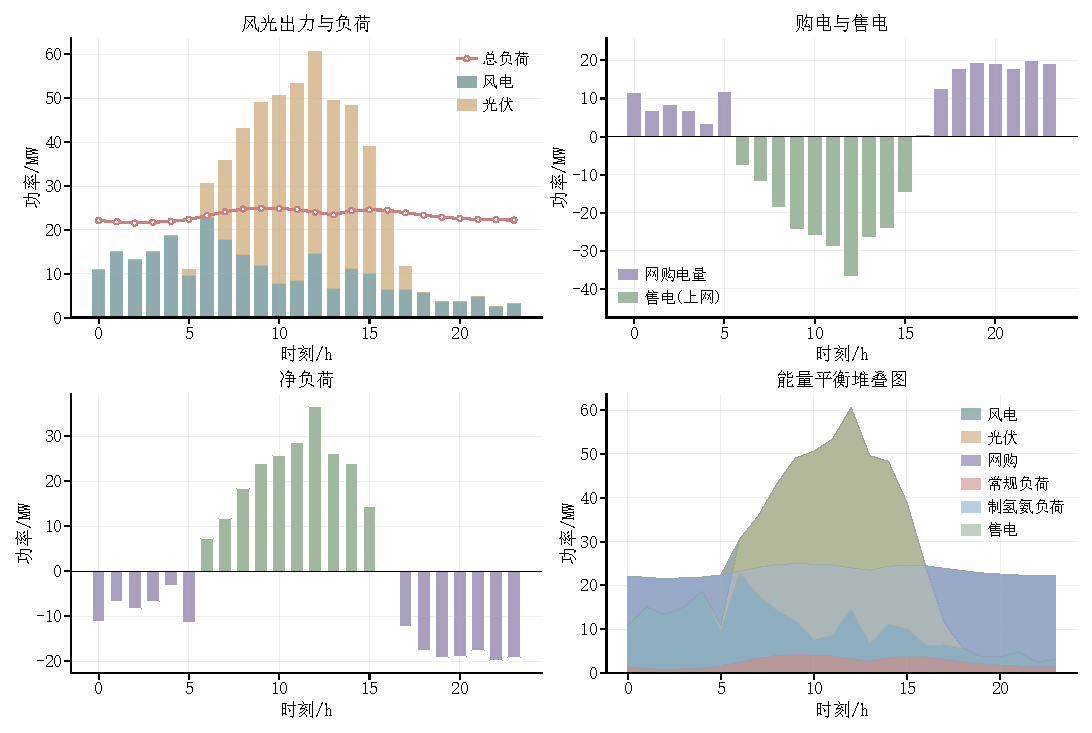
\includegraphics[width=\textwidth]{../figures/q1/fig1_power_balance.pdf}
\caption{园区典型日功率平衡曲线}
\label{fig:q1_balance}
\end{figure}

\cref{fig:q1_balance}从四个维度展示了功率平衡情况：(a)为风电、光伏出力和总负荷的对比，光伏在10:00-14:00出力最大（峰值约46 MW），风电在凌晨和傍晚相对较强（峰值约23 MW）；(b)为购电和售电功率，可见夜间和午间有余电上网，傍晚负荷高峰且光伏归零时需网购电力；(c)为净负荷曲线，正值为余电、负值为缺电，清晰反映了购售电交替规律；(d)为能量平衡堆叠图。

由步骤三和步骤四得到全日能量指标和绿电指标，汇总于\cref{tab:q1_indicators}。

\begin{table}[H]
\centering
\caption{问题一：绿电直连指标与成本}
\label{tab:q1_indicators}
\begin{tabular*}{\textwidth}{@{\extracolsep{\fill}}lcc}
\toprule[1.5pt]
指标 & 计算值 & 要求 \\
\midrule[1pt]
新能源发电量$E_{\mathrm{re}}$ & 603.45 MWh & -- \\
总用电量$E_{\mathrm{total}}$ & 558.72 MWh & -- \\
上网电量$E_{\mathrm{sell}}$ & 216.77 MWh & -- \\
网购电量$E_{\mathrm{buy}}$ & 172.04 MWh & -- \\
自发自用比例$R_{\mathrm{sc}}$ & 28.16\% & $\ge 60\%$ $\times$ \\
总用电绿电比例$R_{\mathrm{g}}$ & 69.21\% & $\ge 30\%$ $\checkmark$ \\
上网电量比例$R_{\mathrm{cur}}$ & 35.92\% & $\le 20\%$ $\times$ \\
吨氨成本$C_{\mathrm{NH_3}}$ & 4322.34 元/吨 & -- \\
\bottomrule[1.5pt]
\end{tabular*}
\end{table}

\cref{tab:q1_indicators}和\cref{fig:q1_radar}使用雷达图直观展示了三个指标与要求值的差距。

\begin{figure}[H]
\centering
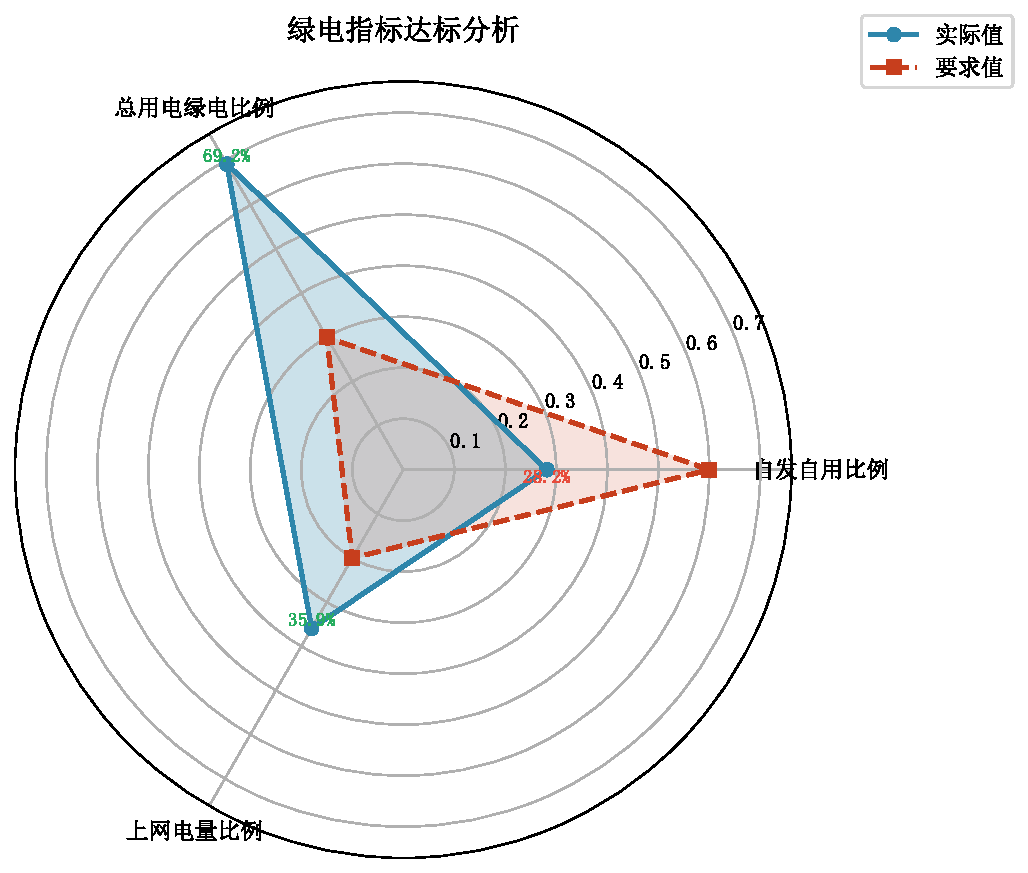
\includegraphics[width=0.55\textwidth]{../figures/q1/fig2_green_indicators_radar.pdf}
\caption{绿电指标达标雷达图}
\label{fig:q1_radar}
\end{figure}

\textbf{原因分析：}三个指标中仅有总用电绿电比例达标（69.21\%），自发自用比例（28.16\%）和上网电量比例（35.92\%）不达标。园区新能源总装机容量104 MW（风电40 MW+光伏64 MW），而制氢氨负荷仅20.75 MW（对应36吨/日产能），总负荷峰值约25 MW。新能源发电能力远超自用需求，大量绿电上网，导致自发自用比例偏低（仅169.91 MWh自用，占发电量的28.16\%）和上网比例偏高（35.92\%）。这一结果表明，36吨/日产能下制氢氨负荷相对于风光装机容量过小，需要通过提升产能或调整可再生能源装机规模来满足绿电直连指标要求\cite{wang2023}。

\section{问题二模型的建立与求解}

\subsection{模型建立}

问题二中园区制氨产能增至72吨/日，制氢氨设备功率按比例线性提升至41.5 MW（ALKEL 20 MW + PEMEL 20 MW + 合成氨装置1.5 MW，产率3.0 t/h）。电氢氨装置只有全额开机和停机两种运行方式，制氨产量从72吨/日起按9吨/日递减至36吨/日。这是一个典型的0-1整数规划问题。

定义0-1变量$x(t) \in \{0,1\}$表示时段$t$是否开机生产：
\begin{equation}
x(t) = \begin{cases}
1, & \text{时段}t\text{开机生产} \\
0, & \text{时段}t\text{停机}
\end{cases} \quad t = 0,1,\ldots,23
\end{equation}

目标为最小化日净电费（购电成本减去售电收益）与运维成本之和：
\begin{equation}
\min \; F = \sum_{t=0}^{23} \bigl[ P_{\mathrm{b}}(t)C_{\mathrm{b}}(t) - P_{\mathrm{s}}(t)C_{\mathrm{s}} + C_{\mathrm{OM}}(t) \bigr] \label{eq:q2_obj}
\end{equation}
当$x(t)=1$时，$P_{\mathrm{prod}}(t)=P_{\mathrm{max}}=41.5$ MW；当$x(t)=0$时，$P_{\mathrm{prod}}(t)=0$。运维成本$C_{\mathrm{OM}}(t) = x(t) \times 5003$元。

约束条件包括功率平衡约束、日产量约束和购售电互斥约束：
\begin{align}
&P_{\mathrm{w}}(t) + P_{\mathrm{pv}}(t) + P_{\mathrm{b}}(t) = P_{\mathrm{L}}(t) + x(t)P_{\mathrm{max}} + P_{\mathrm{s}}(t) \quad \forall t \label{eq:q2_bal} \\
&\sum_{t=0}^{23} x(t) = k,\quad k = Q_{\mathrm{NH_3}}/3 \in \{24,21,18,15,12\} \label{eq:q2_hours} \\
&P_{\mathrm{b}}(t) \ge 0,\; P_{\mathrm{s}}(t) \ge 0,\; P_{\mathrm{b}}(t) \cdot P_{\mathrm{s}}(t) = 0 \quad \forall t
\end{align}

整理为标准整数规划形式：
\begin{align}
\min \; & \sum_{t=0}^{23} \bigl[ C_{\mathrm{b}}(t)\max\{P_{\mathrm{L}}(t) + x(t)P_{\mathrm{max}} - P_{\mathrm{w}}(t) - P_{\mathrm{pv}}(t),\; 0\} \notag \\
&\qquad - C_{\mathrm{s}}\max\{P_{\mathrm{w}}(t) + P_{\mathrm{pv}}(t) - P_{\mathrm{L}}(t) - x(t)P_{\mathrm{max}},\; 0\} + 5003x(t) \bigr] \label{eq:q2_model} \\
\text{s.t.} \quad & \sum_{t=0}^{23} x(t) = k,\; x(t) \in \{0,1\},\; \forall t \notag
\end{align}

\subsection{模型求解}

\textbf{步骤一：确定开机时长。}根据目标日产量$Q_{\mathrm{NH_3}}$，计算所需开机小时数$k = Q_{\mathrm{NH_3}}/3$。72、63、54、45、36吨/日分别对应$k=24,21,18,15,12$小时。

\textbf{步骤二：计算各时段边际成本。}对于每个时段$t=0,\ldots,23$，按以下公式计算相对于不开机而言，开机的边际成本$\Delta C(t)$：
\begin{equation}
\Delta C(t) = \bigl[ C_{\mathrm{on}}(t) - C_{\mathrm{off}}(t) \bigr] + 5003 \label{eq:q2_marginal}
\end{equation}
其中：
\begin{align*}
C_{\mathrm{off}}(t) &=
\begin{cases}
- [P_{\mathrm{w}}(t)+P_{\mathrm{pv}}(t)-P_{\mathrm{L}}(t)] \cdot C_{\mathrm{s}}, & \text{若可再生过剩}\\
[P_{\mathrm{L}}(t)-P_{\mathrm{w}}(t)-P_{\mathrm{pv}}(t)] \cdot C_{\mathrm{b}}(t), & \text{若可再生不足}
\end{cases} \\
C_{\mathrm{on}}(t) &=
\begin{cases}
- [P_{\mathrm{w}}(t)+P_{\mathrm{pv}}(t)-P_{\mathrm{L}}(t)-41.5] \cdot C_{\mathrm{s}}, & \text{若开机后仍过剩}\\
[P_{\mathrm{L}}(t)+41.5-P_{\mathrm{w}}(t)-P_{\mathrm{pv}}(t)] \cdot C_{\mathrm{b}}(t), & \text{若开机后需购电}
\end{cases}
\end{align*}
常数5003元是开机一小时产生的运维费用（ALKEL 20MW$\times$100 + PEMEL 20MW$\times$150 + NH$_3$ 1.5MW$\times$2）。

以$t=12$（12:00-13:00，峰电价0.8024元/kWh）为例：
\begin{align*}
C_{\mathrm{off}}(12) &= -(14.52+46.08-3.26)\times 377.9 = -21\,668\ \text{元} \quad (\text{售电收益})\\
C_{\mathrm{on}}(12) &= -(14.52+46.08-3.26-41.5)\times 377.9 = -5\,985\ \text{元}\\
\Delta C(12) &= (-5\,985) - (-21\,668) + 5\,003 = -10\,680\ \text{元}
\end{align*}
边际成本为负，说明$t=12$开机比停机更省钱（将低价值余电转为氨生产，扣除运维后仍有净收益）。

以$t=19$（19:00-20:00，峰电价0.8024元/kWh）为例：
\begin{align*}
C_{\mathrm{off}}(19) &= (2.12-3.69)\times 0 = 0\ \text{元} \quad (\text{无可再生能源，但净负荷为负})\\
C_{\mathrm{on}}(19) &= (2.12+41.5-3.69)\times 802.4 = 32\,088\ \text{元}\\
\Delta C(19) &= 32\,088 - 0 + 5\,003 = 37\,091\ \text{元}
\end{align*}
边际成本很高，说明$t=19$开机需大量购电，成本极高。

\textbf{步骤三：选择最优时段。}将24个$\Delta C(t)$从小到大排序，选择前$k$个最小的时段开机。以36吨/日（$k=12$）为例，边际成本最低的12个时段集中在10:00-21:00（太阳能充足或风能较好的时段），而夜间和清晨因光伏为零且风电不够支撑满负荷，边际成本较高，因此不开机。

\textbf{步骤四：计算指标和成本。}根据选定的开机方案，计算购售电功率，然后按模型建立部分的公式计算绿电指标和吨氨成本。各产量结果如\cref{tab:q2_typical}所示。

\begin{table}[H]
\centering
\caption{典型场景各产量运行指标}
\label{tab:q2_typical}
\begin{tabular*}{\textwidth}{@{\extracolsep{\fill}}ccccccc}
\toprule[1.5pt]
产量(t/d) & 时长(h) & 成本(元/吨) & 自用比例 & 绿电比例 & 上网比例 & 达标 \\
\midrule[1pt]
72 & 24 & 6219 & 86.5\% & 53.3\% & 6.7\% & $\checkmark$ \\
63 & 21 & 5328 & 84.3\% & 59.7\% & 7.8\% & $\checkmark$ \\
54 & 18 & 4591 & 80.2\% & 67.3\% & 9.9\% & $\checkmark$ \\
45 & 15 & 3945 & 51.0\% & 66.7\% & 24.5\% & $\times$ \\
36 & 12 & 3192 & 10.5\% & 59.7\% & 44.7\% & $\times$ \\
\bottomrule[1.5pt]
\end{tabular*}
\end{table}

\cref{tab:q2_typical}展示了各产量下的成本与绿电指标。随着产量降低，运行小时数减少，购电量也随之下降，使得吨氨成本从72 t/d的6219元/吨降至36 t/d的3192元/吨。然而，低产量下自发自用比例也大幅下滑——36 t/d时仅10.5\%（不满足60\%要求），而上网比例达到44.7\%（不满足20\%要求），说明离散调节下低产工况难以兼顾经济性与绿电指标。

为进一步分析开机策略，根据各产量的最优开机时段绘制甘特图如\cref{fig:q2_gantt}所示。

\begin{figure}[H]
\centering
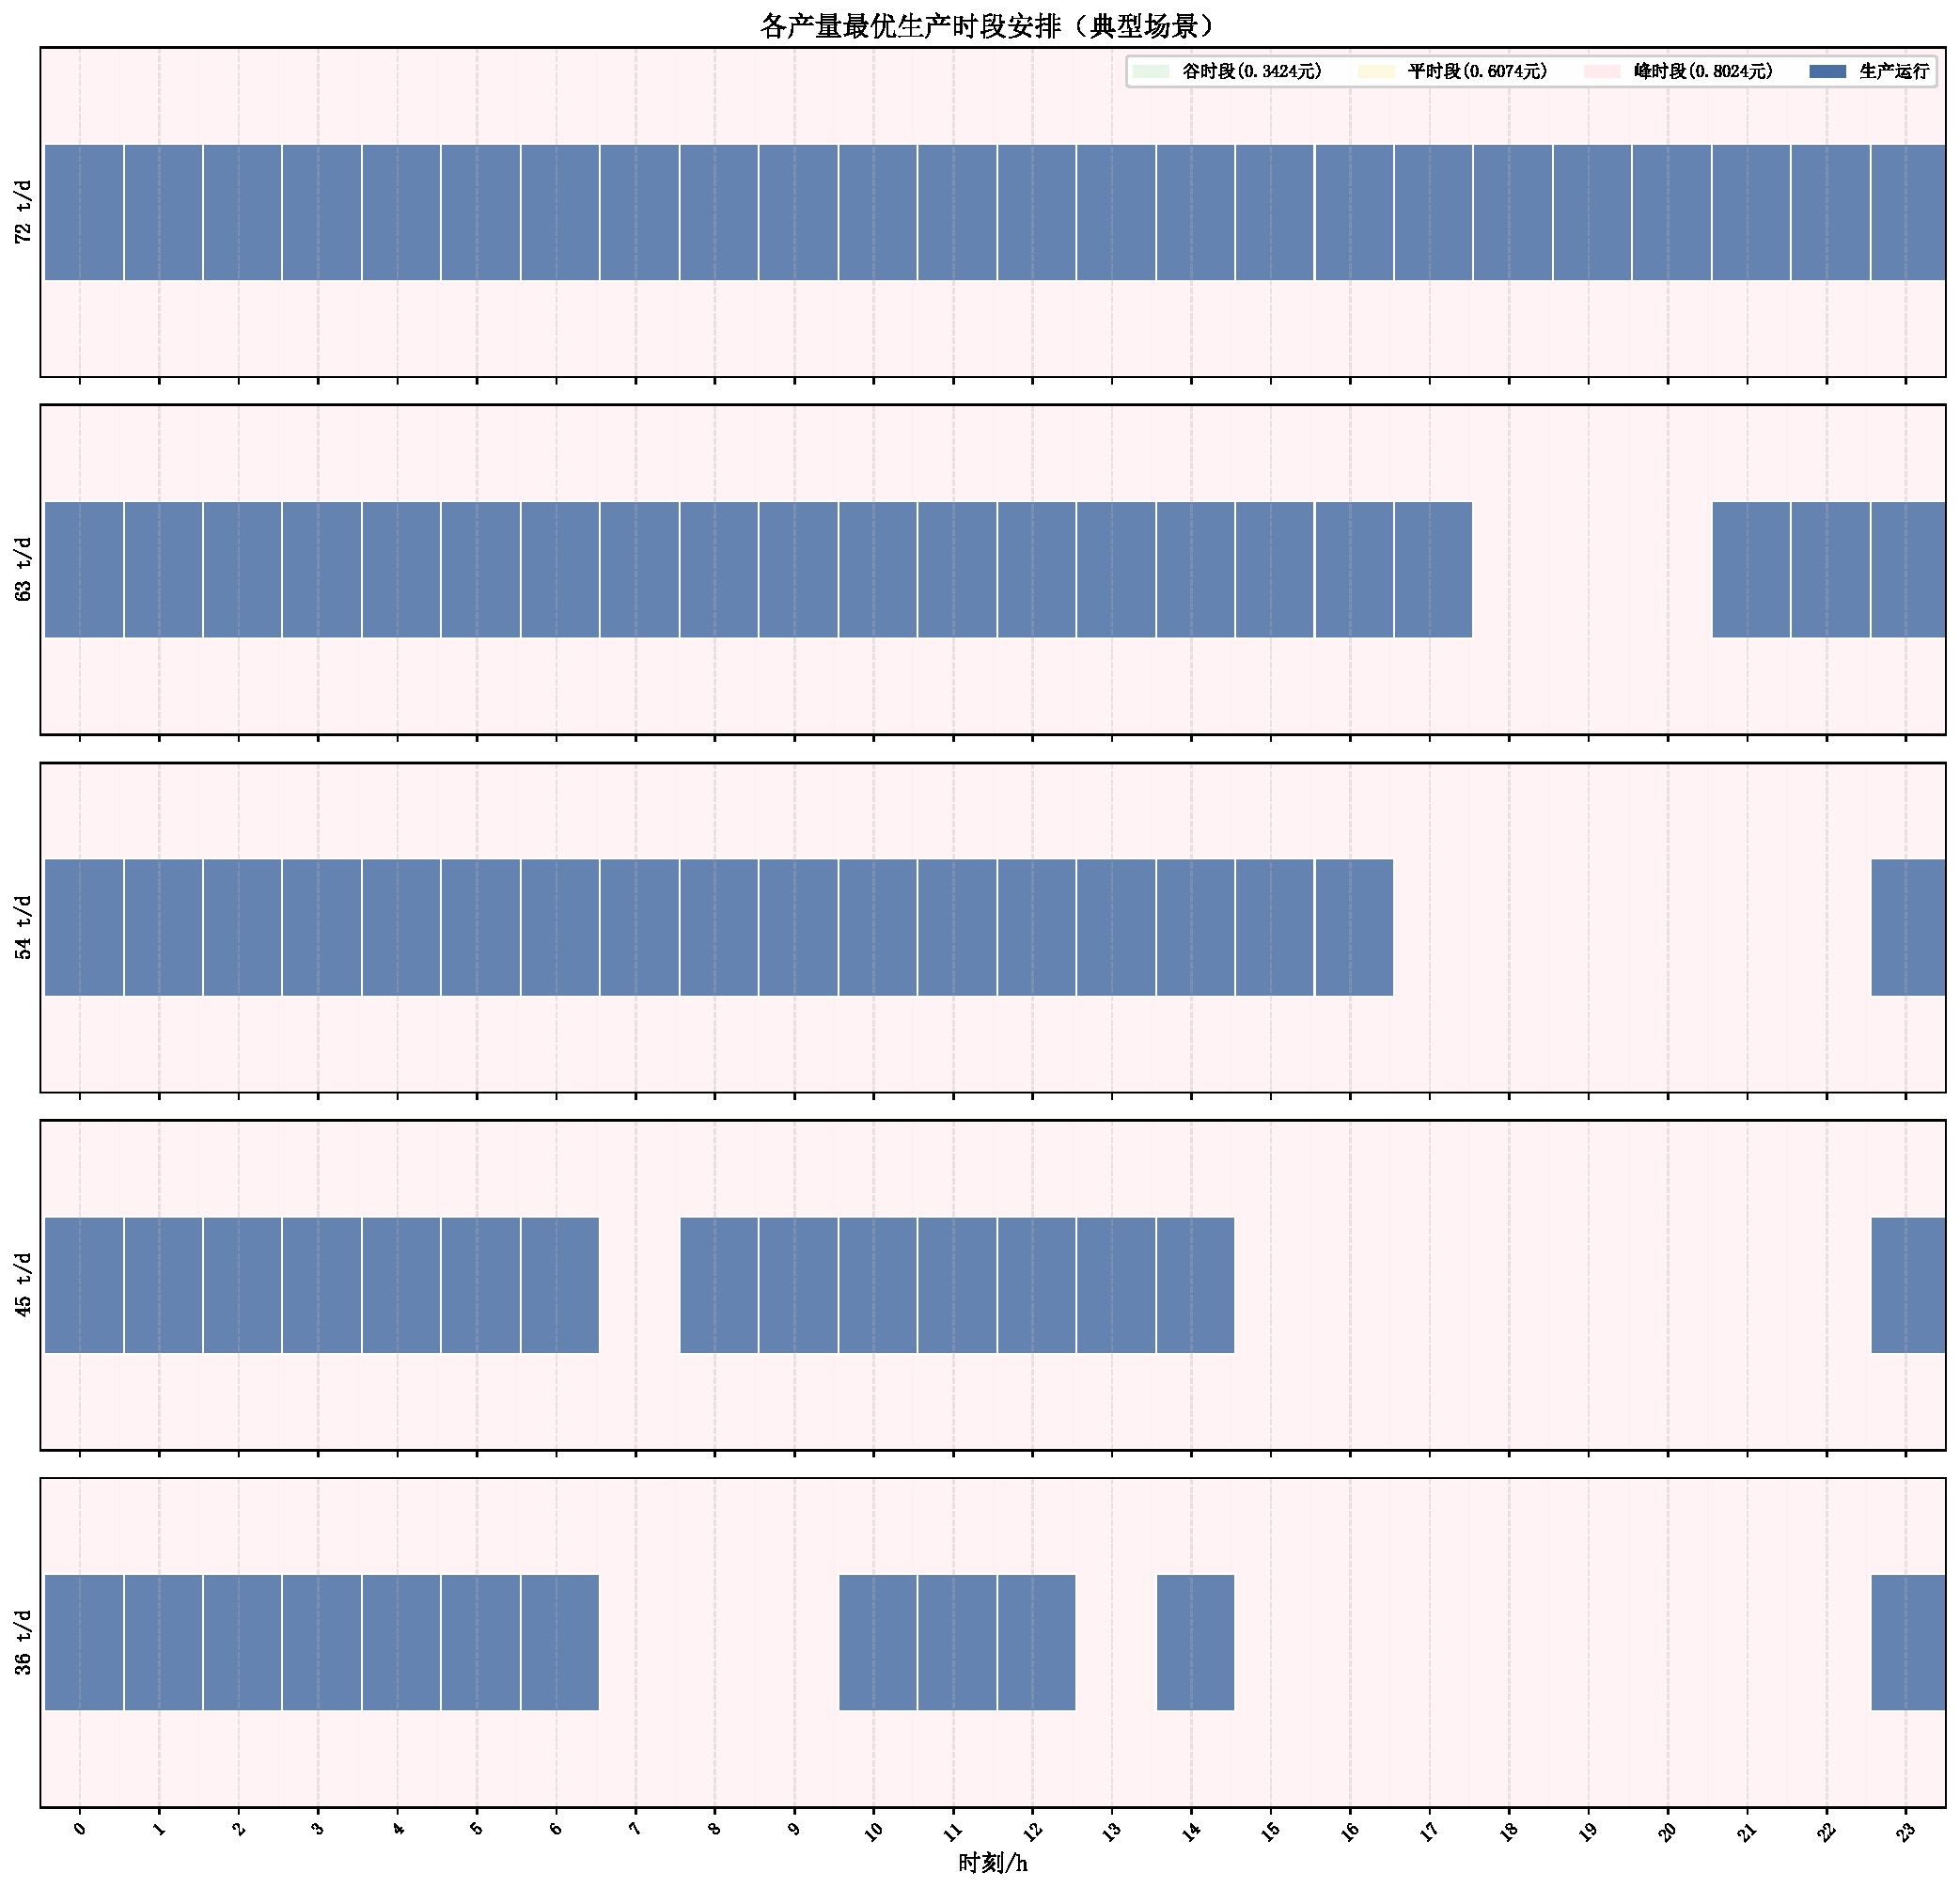
\includegraphics[width=\textwidth]{../figures/q2/fig4_gantt.pdf}
\caption{各产量最优生产时段安排}
\label{fig:q2_gantt}
\end{figure}

\cref{fig:q2_gantt}展示了各产量下最优的24小时开机方案（蓝色条）与电价时段（谷时段绿色、平时段黄色、峰时段粉红）的关系。72 t/d需满发24h，无法选择；63 t/d优先关停了18:00-20:00峰时段（此时光伏归零而负荷攀升，购电成本高达0.8024元/kWh）；54 t/d、45 t/d、36 t/d依次继续关停成本最高的时段，优先保留谷电价时段（0.3424元/kWh）和光伏大发的中午时段。这表明边际成本排序算法倾向于在低价时段和高可再生时段安排生产，有效降低了购电成本。

由各产量的成本和绿电指标数据得到\cref{fig:q2_cvp}。

\begin{figure}[H]
\centering
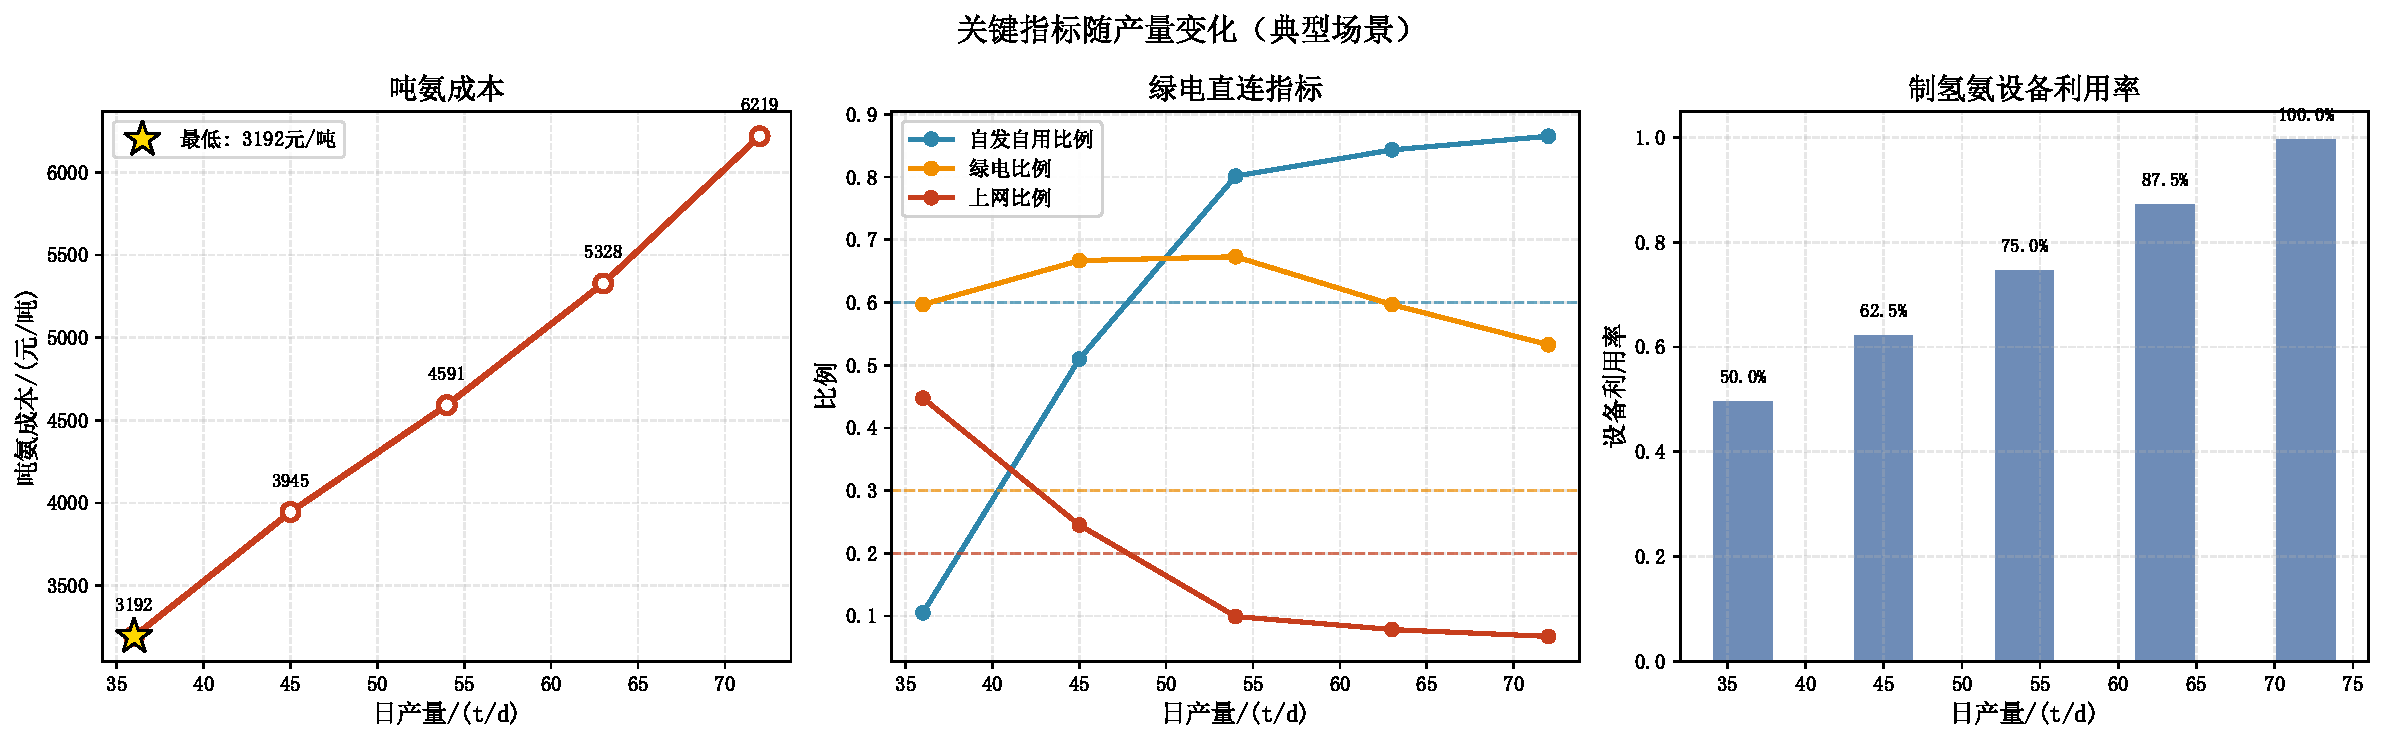
\includegraphics[width=\textwidth]{../figures/q2/fig5_cost_vs_production.pdf}
\caption{关键指标随产量变化}
\label{fig:q2_cvp}
\end{figure}

\cref{fig:q2_cvp}包含三个子图。(a)吨氨成本曲线：从72 t/d的6,219元/吨单调下降至36 t/d的3,192元/吨，降幅约49\%。这是因为低产量下设备运行时间短，购电费用减少、售电收益增加，单位成本被摊薄。(b)绿电指标曲线：自用比例在72-54 t/d时稳定在80\%以上，但45 t/d时骤降至51.0\%（低于60\%要求），36 t/d时进一步降至10.5\%。上网比例在54 t/d时仅9.9\%（达标），45 t/d时升至24.5\%（超标）。这表明离散调节下低产量时大部分可再生电力被上网出售而非自用，导致指标恶化。(c)设备利用率：随产量线性降低，从100\%降至50\%。

以上分析均基于典型日风光出力场景。然而园区实际运行中风光出力具有显著的随机波动性——风电可能全天低于额定功率的10\%，光伏可能因多云天气出力减半。为全面评估离散调节方案在不同天气条件下的表现，将附件3的6种风电场景与附件4的4种光伏场景进行两两组合，共得到24种风光出力场景（如S1风1光1、S2风1光2、…、S24风6光4）。对每种场景重复上述边际成本优化，计算各产量水平下的吨氨成本，绘制热力图如\cref{fig:q2_heatmap}所示。

\begin{figure}[H]
\centering
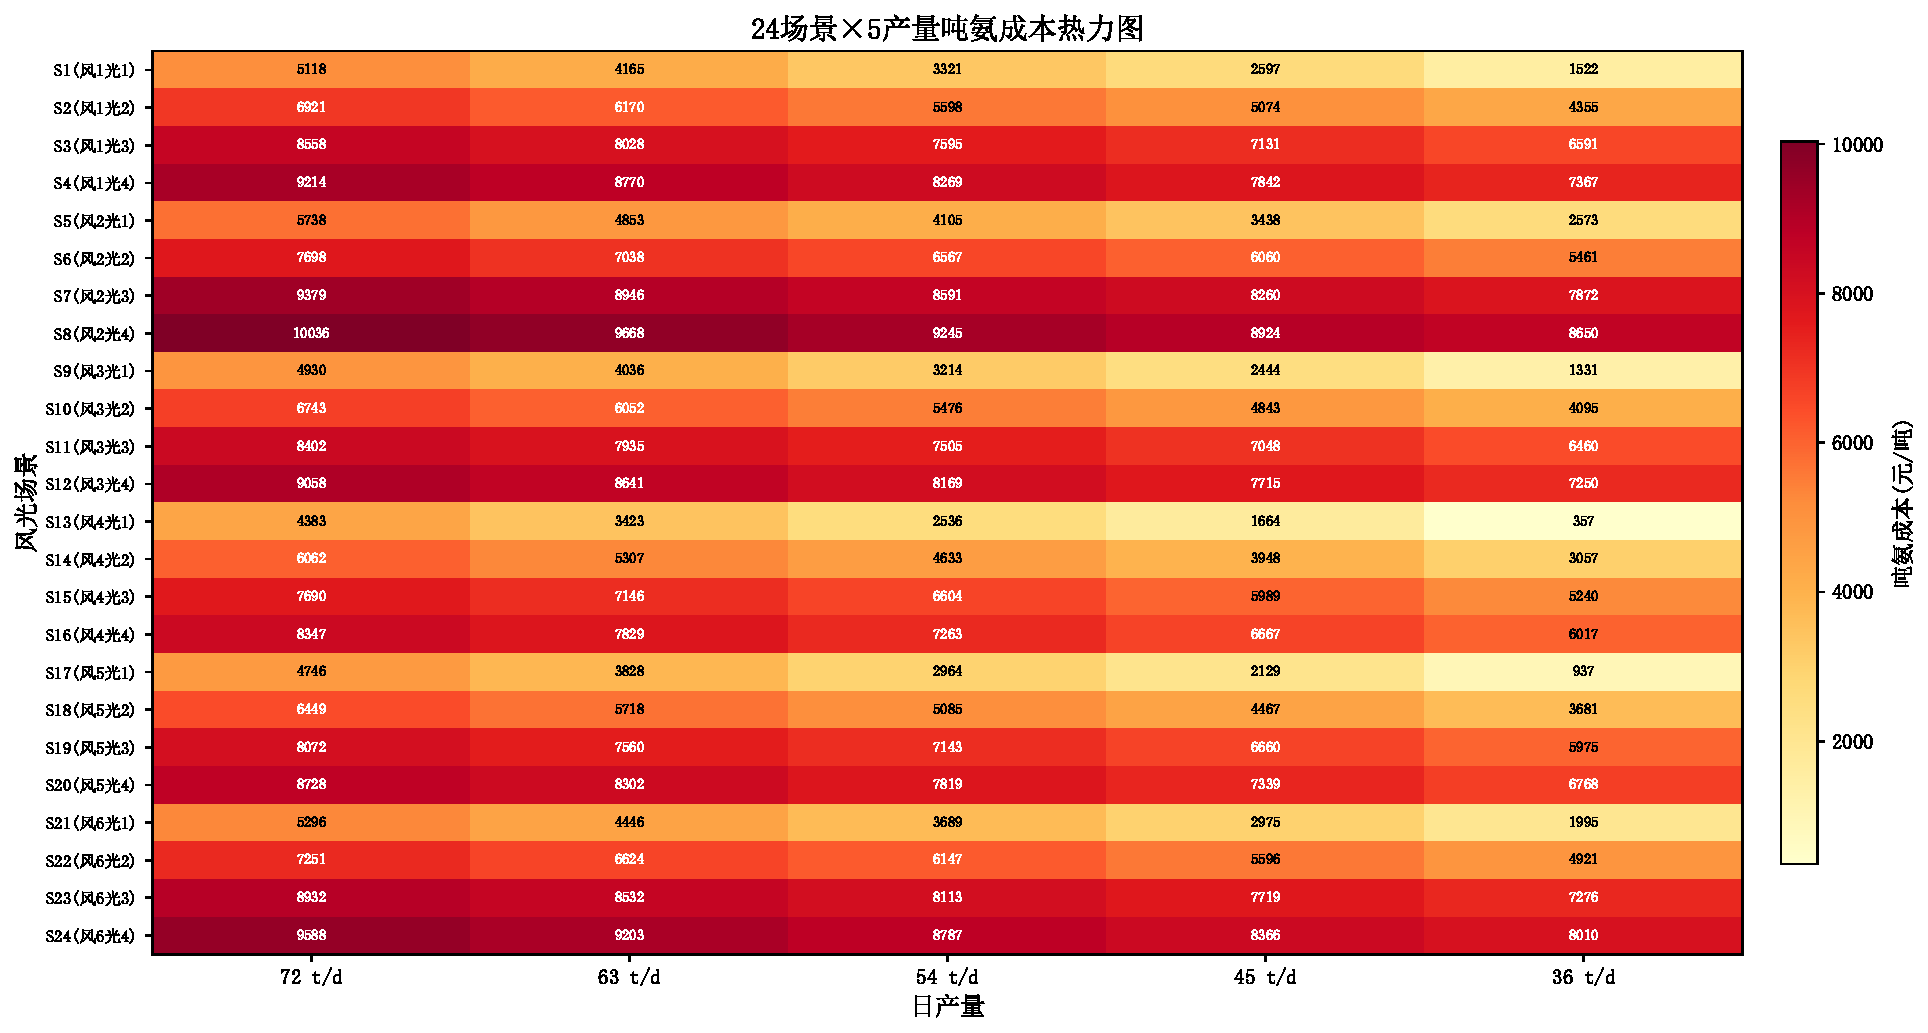
\includegraphics[width=\textwidth]{../figures/q2/fig6_heatmap.pdf}
\caption{24场景$\times$5产量吨氨成本热力图}
\label{fig:q2_heatmap}
\end{figure}

\cref{fig:q2_heatmap}中每一行代表一种风光场景，每一列代表一个产量水平，颜色深浅反映吨氨成本高低。场景S8（风2光4，风电和光伏均偏低）在所有产量下成本均为最高，原因是该场景可再生发电总量少，需大量网购高价电力；场景S13（风4光1，风电高光伏中等）成本最低，因为风电在夜间和全天持续出力。高产量时各场景间成本差异较小（约1,000-2,000元/吨），低产量时差异显著增大（可达5,000元/吨以上），说明低产量下风光条件对经济性的影响更为敏感。

各产量下24种场景的绿电指标达标情况统计如\cref{fig:q2_compliance}所示。

\begin{figure}[H]
\centering
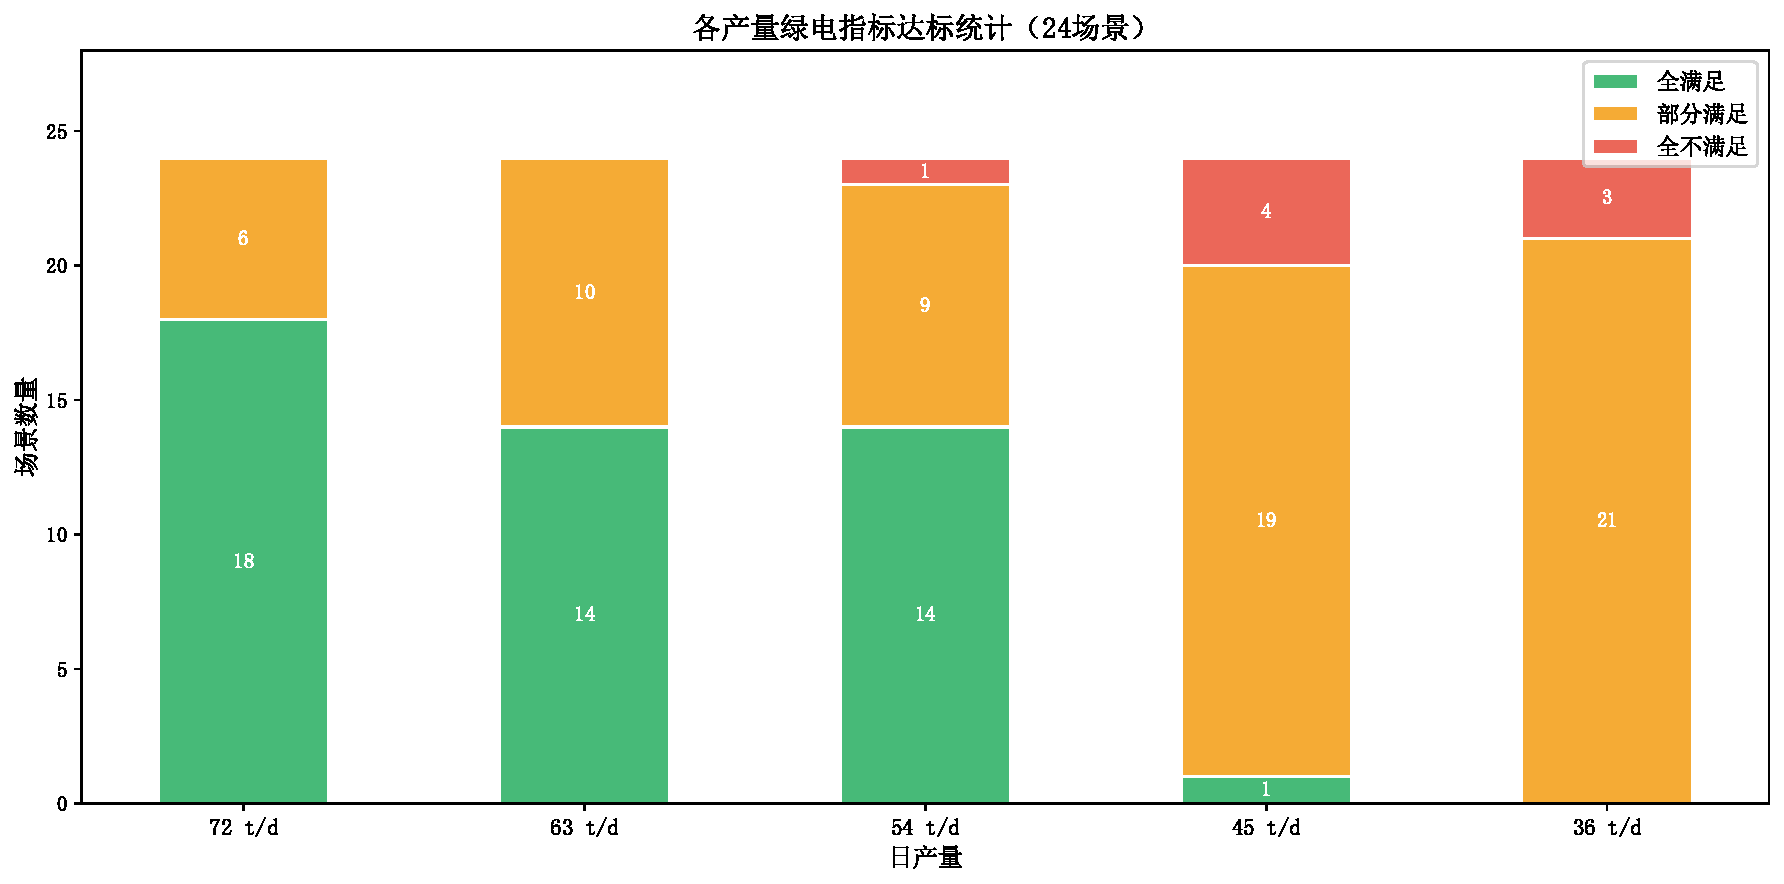
\includegraphics[width=\textwidth]{../figures/q2/fig7_compliance.pdf}
\caption{各产量绿电指标达标统计}
\label{fig:q2_compliance}
\end{figure}

\cref{fig:q2_compliance}按全满足（绿）、部分满足（黄）、全不满足（红）三类统计了24场景的达标情况。72 t/d时18个场景全满足、6个部分满足，表现最好；63 t/d和54 t/d分别有14个全满足，仍属良好；45 t/d时仅1个全满足、19个部分满足、4个全不满足，急剧恶化；36 t/d时0个全满足、21个部分满足、3个全不满足。这说明离散调节下产量降至45 t/d及以下时，即使针对不同风光场景优化调度，也无法使大多数场景的绿电指标达标。根本原因是开机时长过短导致可再生自用电量太少、上网比例过高。

\section{问题三模型的建立与求解}

\subsection{模型建立}

问题三将电氢氨装置的运行方式从离散开关改为功率连续可调（下限为额定功率的10\%）。各时段的制氢氨功率$p(t)$可在$[0.1P_{\mathrm{max}}, P_{\mathrm{max}}]$区间内连续调节，也可完全停机（$p(t)=0$）。这是一个连续线性规划问题。

定义连续变量$p(t)$为时段$t$的制氢氨功率：
\begin{equation}
p(t) \in \{0\} \cup [0.1P_{\mathrm{max}},\; P_{\mathrm{max}}], \quad t = 0,1,\ldots,23 \label{eq:q3_var}
\end{equation}
其中$P_{\mathrm{max}} = 41.5$ MW。

目标为最小化日净电费与运维成本之和：
\begin{equation}
\min \; F = \sum_{t=0}^{23} \bigl[ P_{\mathrm{b}}(t)C_{\mathrm{b}}(t) - P_{\mathrm{s}}(t)C_{\mathrm{s}} + C_{\mathrm{OM}}(t) \bigr] \label{eq:q3_obj}
\end{equation}
运维成本$C_{\mathrm{OM}}(t) = p(t) \times 126$元。

约束条件包括功率平衡、功率上下限和日产量约束：
\begin{align}
&P_{\mathrm{w}}(t) + P_{\mathrm{pv}}(t) + P_{\mathrm{b}}(t) = P_{\mathrm{L}}(t) + p(t) + P_{\mathrm{s}}(t) \quad \forall t \label{eq:q3_bal} \\
&p(t) \in \{0\} \cup [0.1P_{\mathrm{max}},\; P_{\mathrm{max}}] \quad \forall t \label{eq:q3_plim} \\
&\sum_{t=0}^{23} p(t) \cdot \eta = Q_{\mathrm{NH_3}}, \quad \eta = \frac{3.0}{41.5} = 0.0723 \; [\text{t/MWh}] \label{eq:q3_q}
\end{align}

整理为标准形式：
\begin{align}
\min \; & \sum_{t=0}^{23} \Bigl[ C_{\mathrm{b}}(t)\max\{P_{\mathrm{L}}(t) + p(t) - P_{\mathrm{w}}(t) - P_{\mathrm{pv}}(t),\; 0\} \notag \\
&\qquad - C_{\mathrm{s}}\max\{P_{\mathrm{w}}(t) + P_{\mathrm{pv}}(t) - P_{\mathrm{L}}(t) - p(t),\; 0\} + 126p(t) \Bigr] \label{eq:q3_model} \\
\text{s.t.} \quad & \sum_{t=0}^{23} p(t) \cdot \eta = Q_{\mathrm{NH_3}},\; p(t) \in \{0\} \cup [0.1P_{\mathrm{max}},\; P_{\mathrm{max}}],\; \forall t \notag
\end{align}

\subsection{模型求解}

\textbf{步骤一：计算各时段可再生盈余。}对每个时段$t$，计算风光出力扣除常规负荷后的剩余功率：
\begin{equation*}
\Delta P(t) = \max\{0,\; P_{\mathrm{w}}(t) + P_{\mathrm{pv}}(t) - P_{\mathrm{L}}(t)\}
\end{equation*}
这个盈余是可免费利用的可再生电力（若不利用只能以0.3779元/kWh的价格上网出售）。

\textbf{步骤二：优先利用盈余。}将盈余最大的时段按从大到小排序，逐时段分配制氢功率$p(t)$。对于每个时段，尽量利用盈余，但不超过设备最大功率41.5 MW且不低于最小功率4.15 MW：
\begin{equation*}
p(t) = \min\{\text{剩余需求},\; \Delta P(t),\; 41.5\}
\end{equation*}
若$\Delta P(t) < 4.15$ MW，则不在此时段分配功率（无法满足下限要求）。

\textbf{步骤三：不足部分按边际成本分配。}如果步骤二分配后仍有剩余产量需求，计算剩余时段开机的边际成本：
\begin{equation*}
\text{边际成本} = 
\begin{cases}
-377.9 + 126 = -251.9\ \text{元/MWh}, & \text{该时段可再生有盈余}\\
C_{\mathrm{b}}(t) + 126\ \text{元/MWh}, & \text{该时段需购电}
\end{cases}
\end{equation*}
其中$-377.9$是放弃售电的机会成本，$+126$是运维成本。按边际成本从小到大排序，逐时段分配功率。

以36吨/日目标为例，先分配盈余时段：
\begin{itemize}
    \item $t=12$，$\Delta P=57.3$ MW，可取满41.5 MW
    \item $t=11$，$\Delta P=50.1$ MW，可取满41.5 MW
    \item 依次分配盈余时段后，仍有少量剩余需求
\end{itemize}
然后将剩余需求量按边际成本最小的原则分配到$t=0-6$谷电价时段（购电价342.4元/MWh$+126=468.4$元/MWh）。

\textbf{步骤四：微调余量。}若最后剩余不足4.15 MW的功率需求，追加到已有运行时段上（在其现有功率基础上增加少量出力，确保总功率不超过41.5 MW），保证产量精确达标。

为了直观展示连续调节与离散调节在调度策略上的本质差异，以72吨/日满产为例，分别运行两种优化算法得到各时段的制氢氨功率安排、购电功率和售电功率，绘制对比图如\cref{fig:q3_schedule}所示。其中离散调节的功率曲线呈阶梯状（要么满发41.5 MW，要么停机0 MW），连续调节的功率曲线可连续变化。

\begin{figure}[H]
\centering
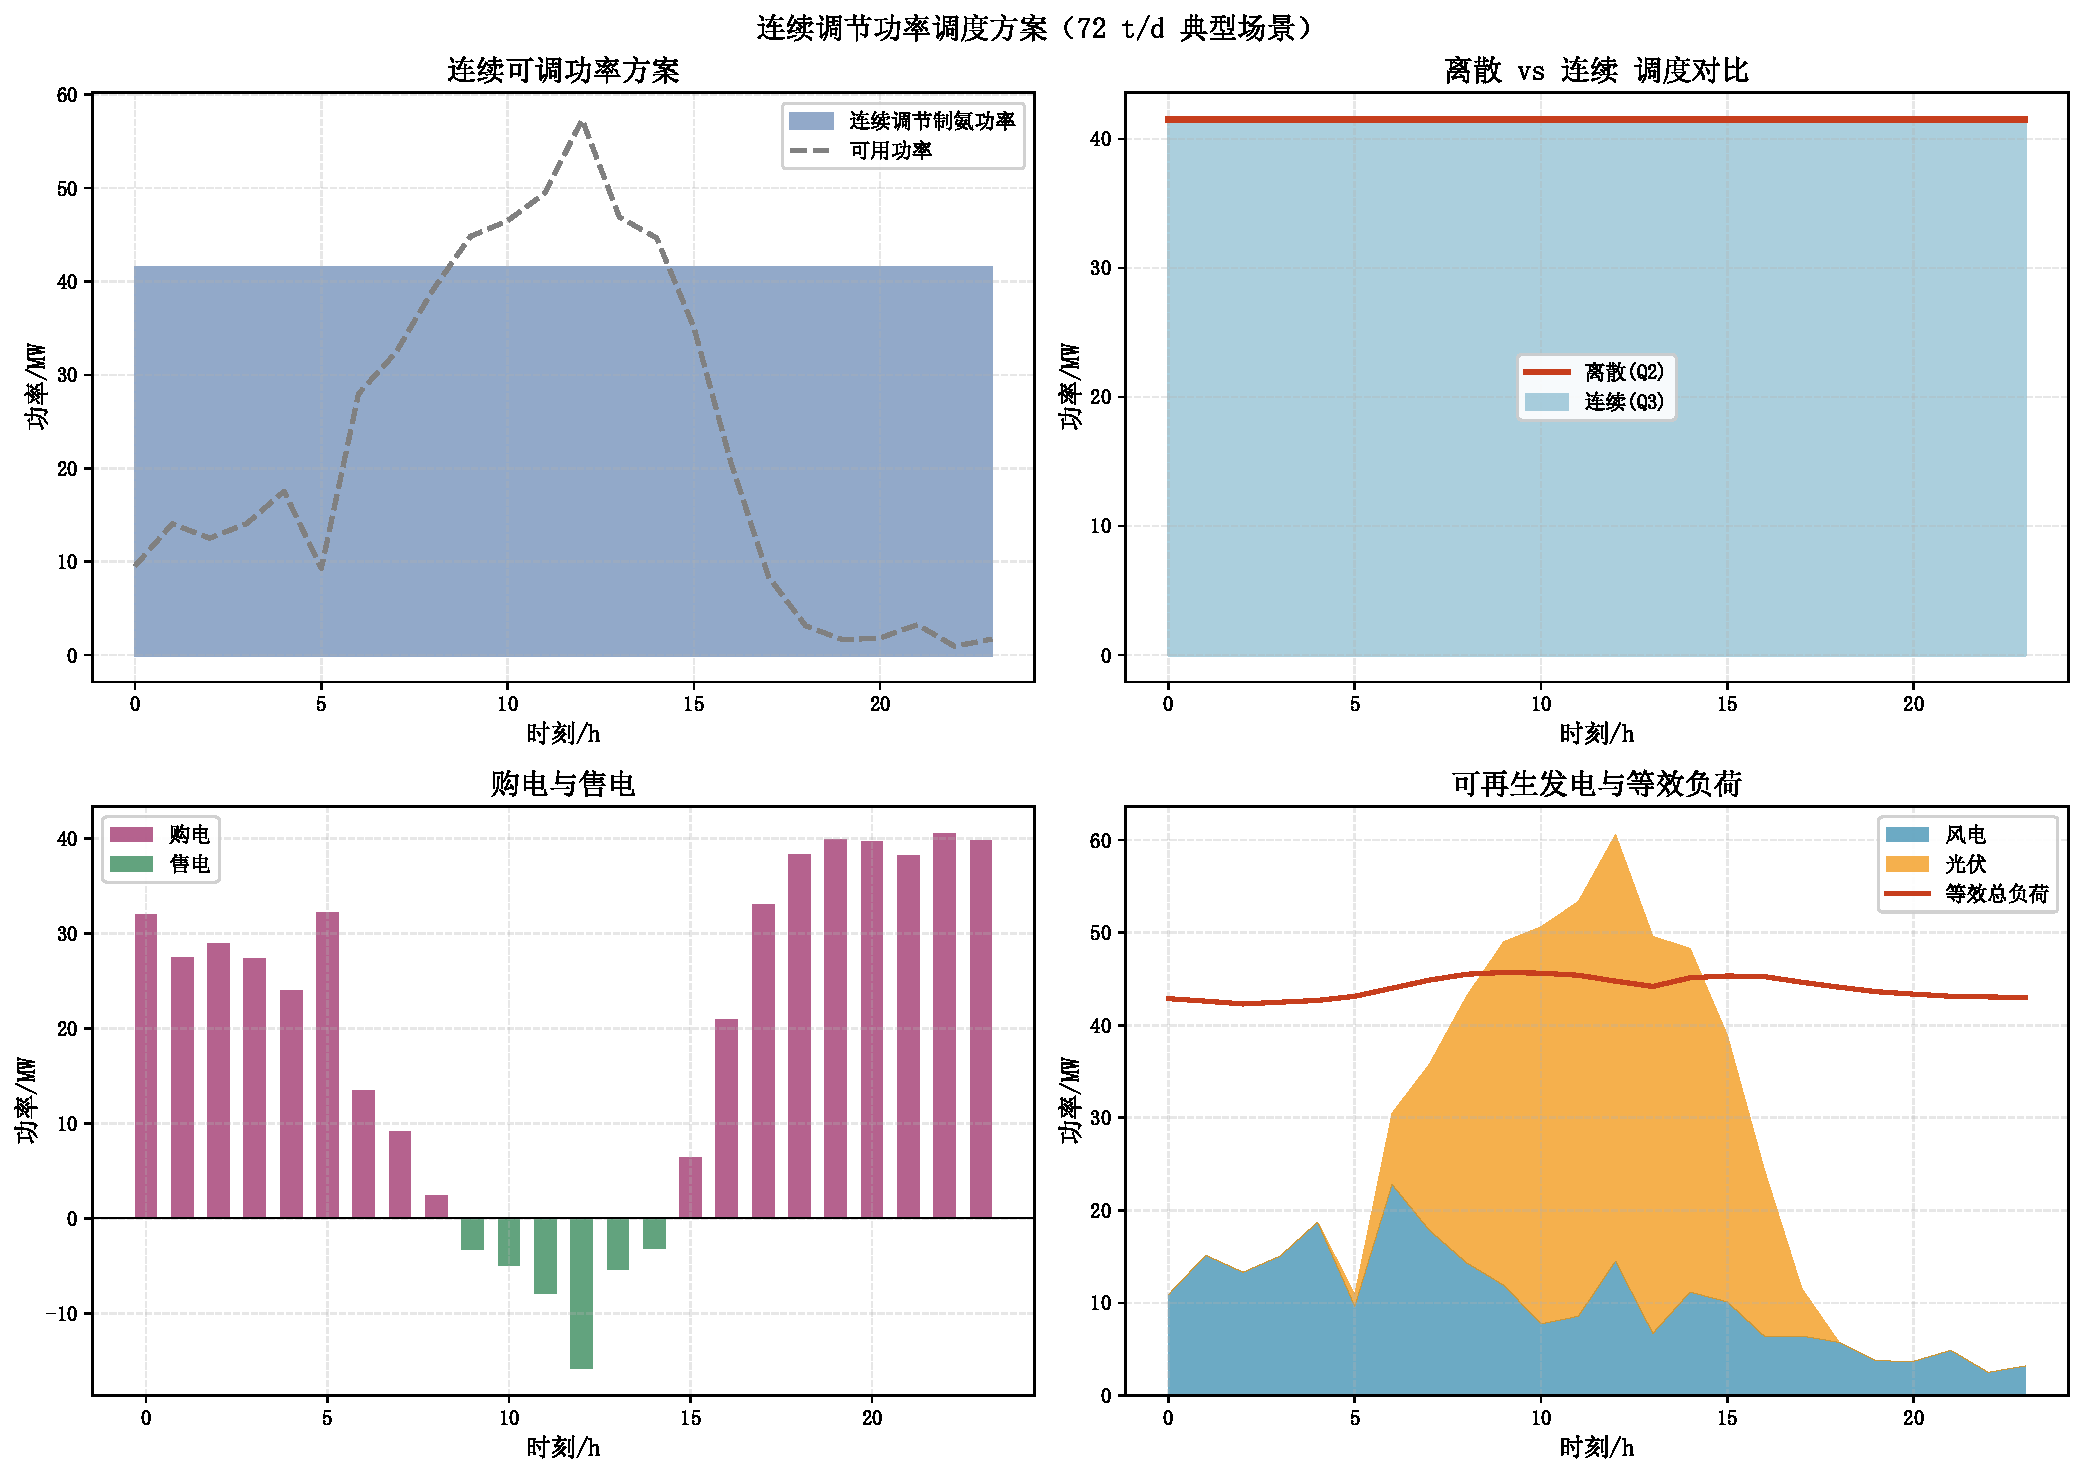
\includegraphics[width=\textwidth]{../figures/q3/fig9_q3_power_schedule.pdf}
\caption{连续调节功率调度方案（72 t/d典型场景）}
\label{fig:q3_schedule}
\end{figure}

\cref{fig:q3_schedule}对比了同一场景下离散和连续调节的差异。连续调节的制氨功率平滑跟随可再生出力，避免了购售电极端波动。

各产量下Q2与Q3的关键指标对比见\cref{tab:q3_comparison}。

\begin{table}[H]
\centering
\caption{Q2与Q3关键指标对比（典型场景）}
\label{tab:q3_comparison}
\begin{tabular*}{\textwidth}{@{\extracolsep{\fill}}ccccccc}
\toprule[1.5pt]
产量 & \multicolumn{2}{c}{吨氨成本(元/吨)} & \multicolumn{2}{c}{自用比例} & \multicolumn{2}{c}{上网比例} \\
(t/d) & Q2 & Q3 & Q2 & Q3 & Q2 & Q3 \\
\midrule[1pt]
72 & 6219 & 6219 & 86.5\% & 86.5\% & 6.7\% & 6.7\% \\
63 & 5328 & 5858 & 84.3\% & 84.6\% & 7.8\% & 7.7\% \\
54 & 4591 & 4758 & 80.2\% & 82.4\% & 9.9\% & 8.8\% \\
45 & 3945 & 4005 & 51.0\% & 82.4\% & 24.5\% & 8.8\% \\
36 & 3192 & 3406 & 10.5\% & 82.4\% & 44.7\% & 8.8\% \\
\bottomrule[1.5pt]
\end{tabular*}
\end{table}

\cref{tab:q3_comparison}显示连续调节在各产量下自用比例稳定在82\%以上，上网比例控制在9\%以内，显著优于离散调节。

以上对比仅基于典型日场景，不足以全面反映连续调节的优势。为进一步验证连续调节在多种天气条件下的表现，将6种风电场景与4种光伏场景两两组合得到24种风光场景，分别在离散和连续两种调节方式下进行优化。对每种场景的每个产量水平，计算其吨氨成本和绿电指标，与离散调节的结果进行逐场景对比。将各产量下24场景的成本均值和达标情况汇总，绘制Q2与Q3的成本对比图和达标统计对比图如\cref{fig:q10_comparison}和\cref{fig:q12_compliance}所示。

\begin{figure}[H]
\centering
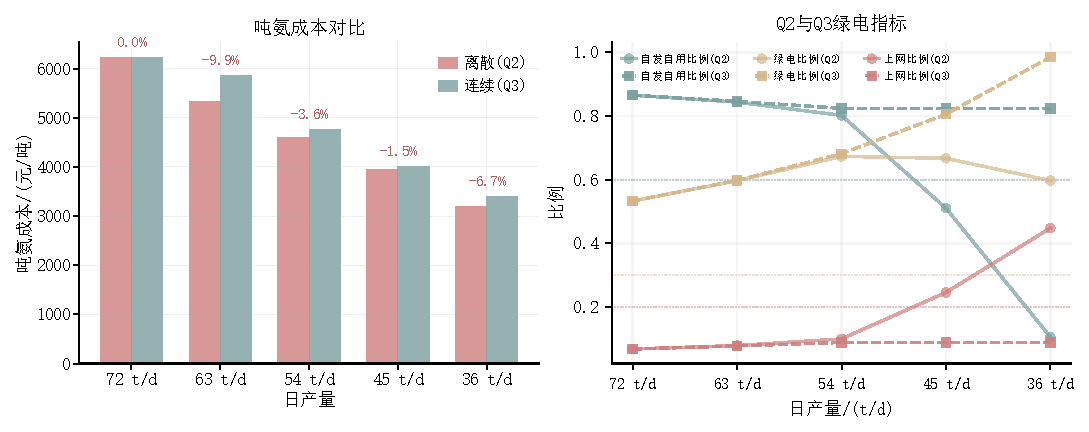
\includegraphics[width=\textwidth]{../figures/q3/fig10_q2_vs_q3.pdf}
\caption{Q2 vs Q3吨氨成本与绿电指标对比}
\label{fig:q10_comparison}
\end{figure}

\begin{figure}[H]
\centering
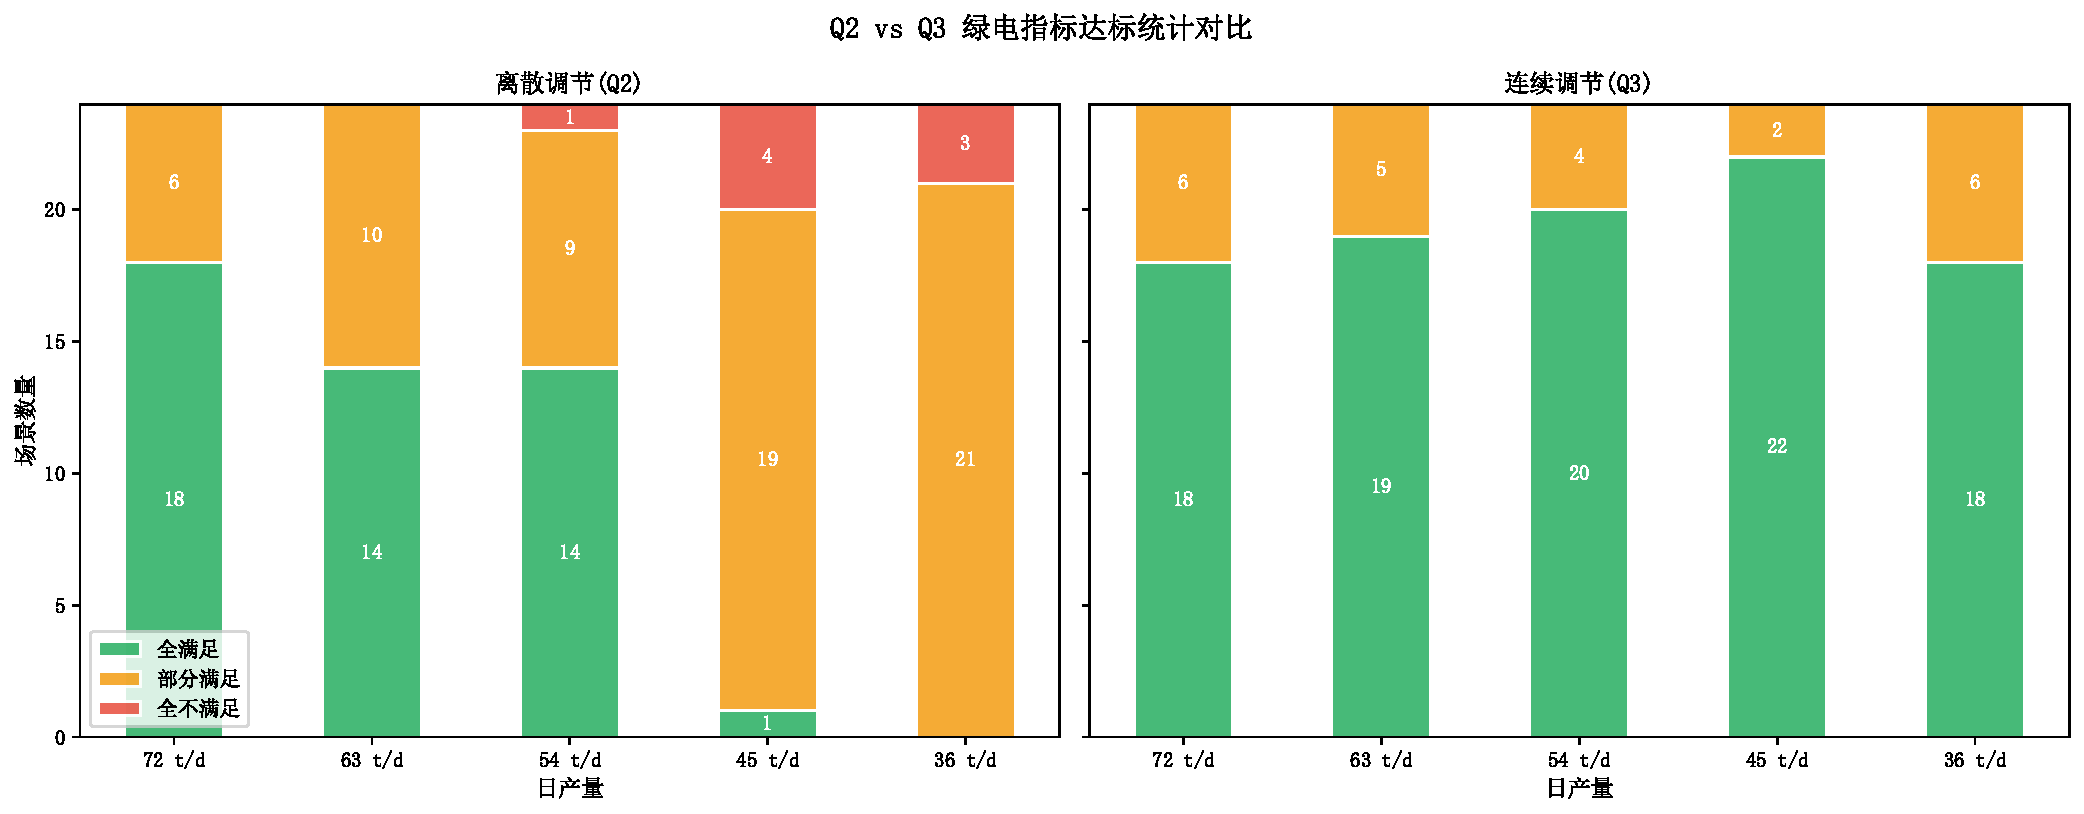
\includegraphics[width=\textwidth]{../figures/q3/fig12_q3_vs_q2_compliance.pdf}
\caption{Q2 vs Q3绿电指标达标统计对比}
\label{fig:q12_compliance}
\end{figure}

\cref{fig:q10_comparison}从成本角度对比了两种调节方式。连续调节在各产量下的吨氨成本略高于离散调节（约200-400元/吨），这是因为连续调节不再大量出售可再生余电，而是将其用于替代网购电力，虽然增加了自发自用电量、改善了绿电指标，但也减少了售电收益。以45 t/d为例，离散调节下售电收益较高使得成本低至3,945元/吨，但自用比例仅51.0%；连续调节下售电收益减少，成本升至4,005元/吨，但自用比例恢复到82.4%。

\cref{fig:q12_compliance}从达标角度展示了连续调节的压倒性优势。72 t/d时两种方式一致（均为18个全满足），但随着产量降低，离散调节的全满足数量急剧下降（45 t/d仅1个、36 t/d为0个），而连续调节的全满足数始终保持在18-22个的高水平。特别值得注意的是45 t/d这一产量——离散调节仅1个场景全满足，而连续调节高达22个。具体数量如\cref{tab:q3_compliance}所示。

\begin{table}[H]
\centering
\caption{Q2与Q3达标场景数对比}
\label{tab:q3_compliance}
\begin{tabular*}{\textwidth}{@{\extracolsep{\fill}}ccccccc}
\toprule[1.5pt]
产量 & \multicolumn{2}{c}{全满足} & \multicolumn{2}{c}{部分满足} & \multicolumn{2}{c}{全不满足} \\
(t/d) & Q2 & Q3 & Q2 & Q3 & Q2 & Q3 \\
\midrule[1pt]
72 & 18 & 18 & 6 & 6 & 0 & 0 \\
63 & 14 & 19 & 10 & 5 & 0 & 0 \\
54 & 14 & 20 & 9 & 4 & 1 & 0 \\
45 & 1 & 22 & 19 & 2 & 4 & 0 \\
36 & 0 & 18 & 21 & 6 & 3 & 0 \\
\bottomrule[1.5pt]
\end{tabular*}
\end{table}

\section{问题四模型的建立与求解}

\subsection{模型建立}

问题四要求分析园区离网运行时的能源自给状况并研究储能的最优配置。离网运行时园区与公共电网无电气连接（$P_{\mathrm{b}}(t)=P_{\mathrm{s}}(t)\equiv 0$），制氢氨功率必须跟随可再生出力变化。

离网运行下，功率平衡方程为：
\begin{equation}
P_{\mathrm{w}}(t) + P_{\mathrm{pv}}(t) = P_{\mathrm{L}}(t) + P_{\mathrm{prod}}(t) + P_{\mathrm{ch}}(t) - P_{\mathrm{dis}}(t) + P_{\mathrm{cur}}(t) \label{eq:q4_bal}
\end{equation}
其中$P_{\mathrm{cur}}(t)$为弃电功率。无储能时，$P_{\mathrm{ch}}(t)=P_{\mathrm{dis}}(t)\equiv 0$，可用功率$P_{\mathrm{avail}}(t) = \max\{0,\; P_{\mathrm{w}}(t)+P_{\mathrm{pv}}(t)-P_{\mathrm{L}}(t)\}$，制氢氨功率：
\begin{equation}
P_{\mathrm{prod}}(t) = \begin{cases}
P_{\mathrm{max}}, & P_{\mathrm{avail}}(t) \ge P_{\mathrm{max}} \\
P_{\mathrm{avail}}(t), & P_{\mathrm{min}} \le P_{\mathrm{avail}}(t) < P_{\mathrm{max}} \\
0, & P_{\mathrm{avail}}(t) < P_{\mathrm{min}}
\end{cases} \label{eq:q4_prod}
\end{equation}
其中$P_{\mathrm{min}} = 0.1P_{\mathrm{max}} = 4.15$ MW。

储能设备的荷电状态（SOC）动态方程\cite{li2023ieee}为：
\begin{equation}
E(t+1) = E(t)(1-\delta) + P_{\mathrm{ch}}(t)\eta_{\mathrm{ch}} - \frac{P_{\mathrm{dis}}(t)}{\eta_{\mathrm{dis}}} \label{eq:q4_soc}
\end{equation}
其中各参数如\cref{tab:q4_storage_params}所示。约束条件包括$0 \le E(t) \le E_{\mathrm{max}}$、充放电功率限制及充放电互斥。

\begin{table}[H]
\centering
\caption{储能设备参数}
\label{tab:q4_storage_params}
\begin{tabular*}{\textwidth}{@{\extracolsep{\fill}}lc}
\toprule[1.5pt]
参数 & 取值 \\
\midrule[1pt]
自损耗率$\delta$ & 0.2\% \\
充电效率$\eta_{\mathrm{ch}}$ & 90\% \\
放电效率$\eta_{\mathrm{dis}}$ & 90\% \\
投资成本 & 1000 元/kWh \\
使用寿命 & 15 年 \\
\bottomrule[1.5pt]
\end{tabular*}
\end{table}

储能容量优化采用双层模型：外层枚举$E_{\mathrm{max}} \in [0, 200]$ MWh，目标为最小化年均吨氨成本（含储能投资折旧和运维）；内层在每种风光场景下优化逐时调度，使可再生能源利用最大、弃电最小。

\subsection{模型求解}

\textbf{离网无储能求解。}对每个场景$t=0,\ldots,23$：
\begin{enumerate}
    \item 计算可用功率$P_{\mathrm{avail}}(t) = \max\{0,\; P_{\mathrm{w}}(t)+P_{\mathrm{pv}}(t)-P_{\mathrm{L}}(t)\}$。
    \item 若$P_{\mathrm{avail}}(t) \ge 41.5$ MW，取满发$P_{\mathrm{prod}}(t)=41.5$ MW，弃电$P_{\mathrm{cur}}(t)=P_{\mathrm{avail}}(t)-41.5$。
    \item 若$4.15 \le P_{\mathrm{avail}}(t) < 41.5$ MW，按可用功率生产$P_{\mathrm{prod}}(t)=P_{\mathrm{avail}}(t)$，无弃电。
    \item 若$P_{\mathrm{avail}}(t) < 4.15$ MW，无法开机$P_{\mathrm{prod}}(t)=0$，$P_{\mathrm{avail}}(t)$全部弃掉。
\end{enumerate}
由$P_{\mathrm{prod}}(t)$累计日产量：$Q_{\mathrm{day}} = [\sum P_{\mathrm{prod}}(t)] \times 0.0723$。

以S13（风4光1）为例：白天光伏大发时段（10:00-14:00）可再生盈余50-70 MW，制氨满载41.5 MW，多余电量弃掉；夜间和傍晚盈余不足4.15 MW时停机。该场景日产量约46.2吨，弃电177.3 MWh。

\textbf{储能配置求解。}外层枚举储能容量$E_{\mathrm{max}} = 0,20,40,\ldots,200$ MWh，内层调度规则为：
\begin{enumerate}
    \item 有盈余时：先满足生产，剩余电量优先给储能充电（不超过SOC上限和充电功率限制）。
    \item 可再生不足时：若储能SOC足够，放电补充生产，使$P_{\mathrm{prod}}$达到最小开机功率以上。
\end{enumerate}
每个储能容量下计算24场景的年均吨氨成本（含储能折旧和运维），结果如\cref{fig:q15_pareto}所示。

\textbf{离网联网对比求解。}按题目要求，在相同产量下对比。对每个场景取离网产量$Q_{\mathrm{off}}$，调用问题三连续调节模型计算联网模式在同等产量下的成本，然后统计全年均值。

\textbf{结果分析。}由最大弃电场景S13的功率数据绘制离网运行功率平衡图如\cref{fig:q13_offgrid}所示。

\begin{figure}[H]
\centering
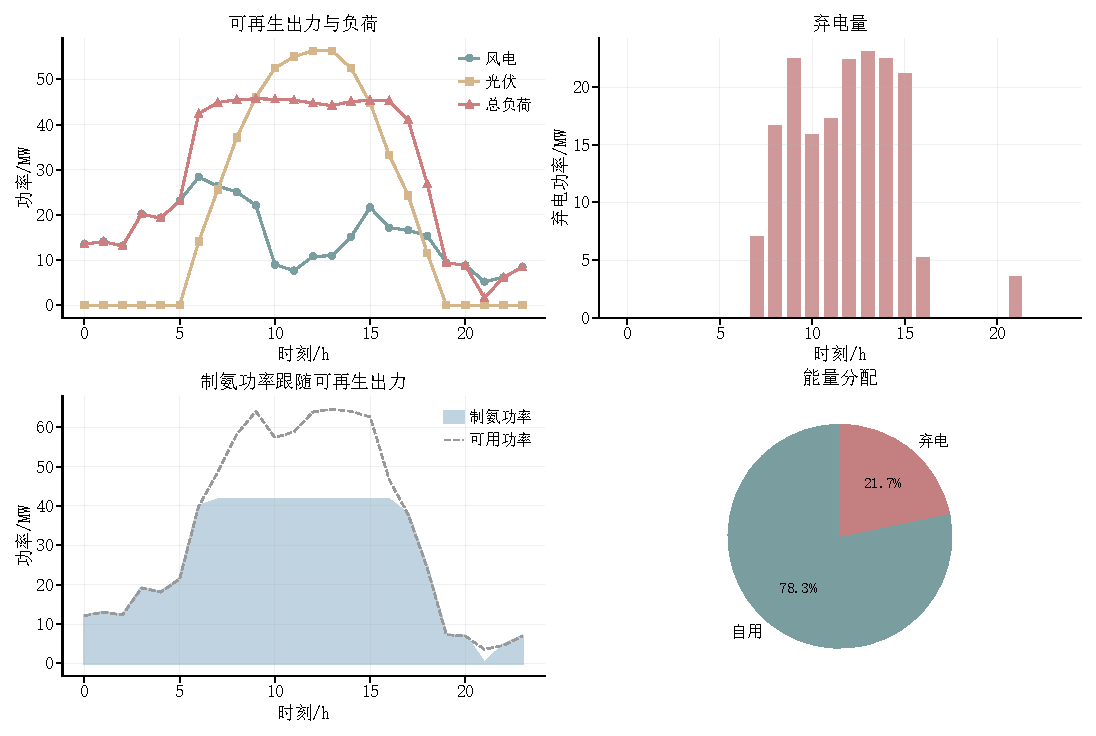
\includegraphics[width=\textwidth]{../figures/q4/fig13_offgrid_power_balance.pdf}
\caption{最大弃电场景（S13风4光1）离网运行功率平衡}
\label{fig:q13_offgrid}
\end{figure}

\cref{fig:q13_offgrid}展示了离网运行时制氨功率紧密跟随可再生出力——白天光伏大发时段制氨功率接近满载，夜间和低出力时段则下降或停机。

24场景的离网产量与弃电率分布如\cref{fig:q14_prod_curtail}所示，汇总指标见\cref{tab:q4_1}。

\begin{figure}[H]
\centering
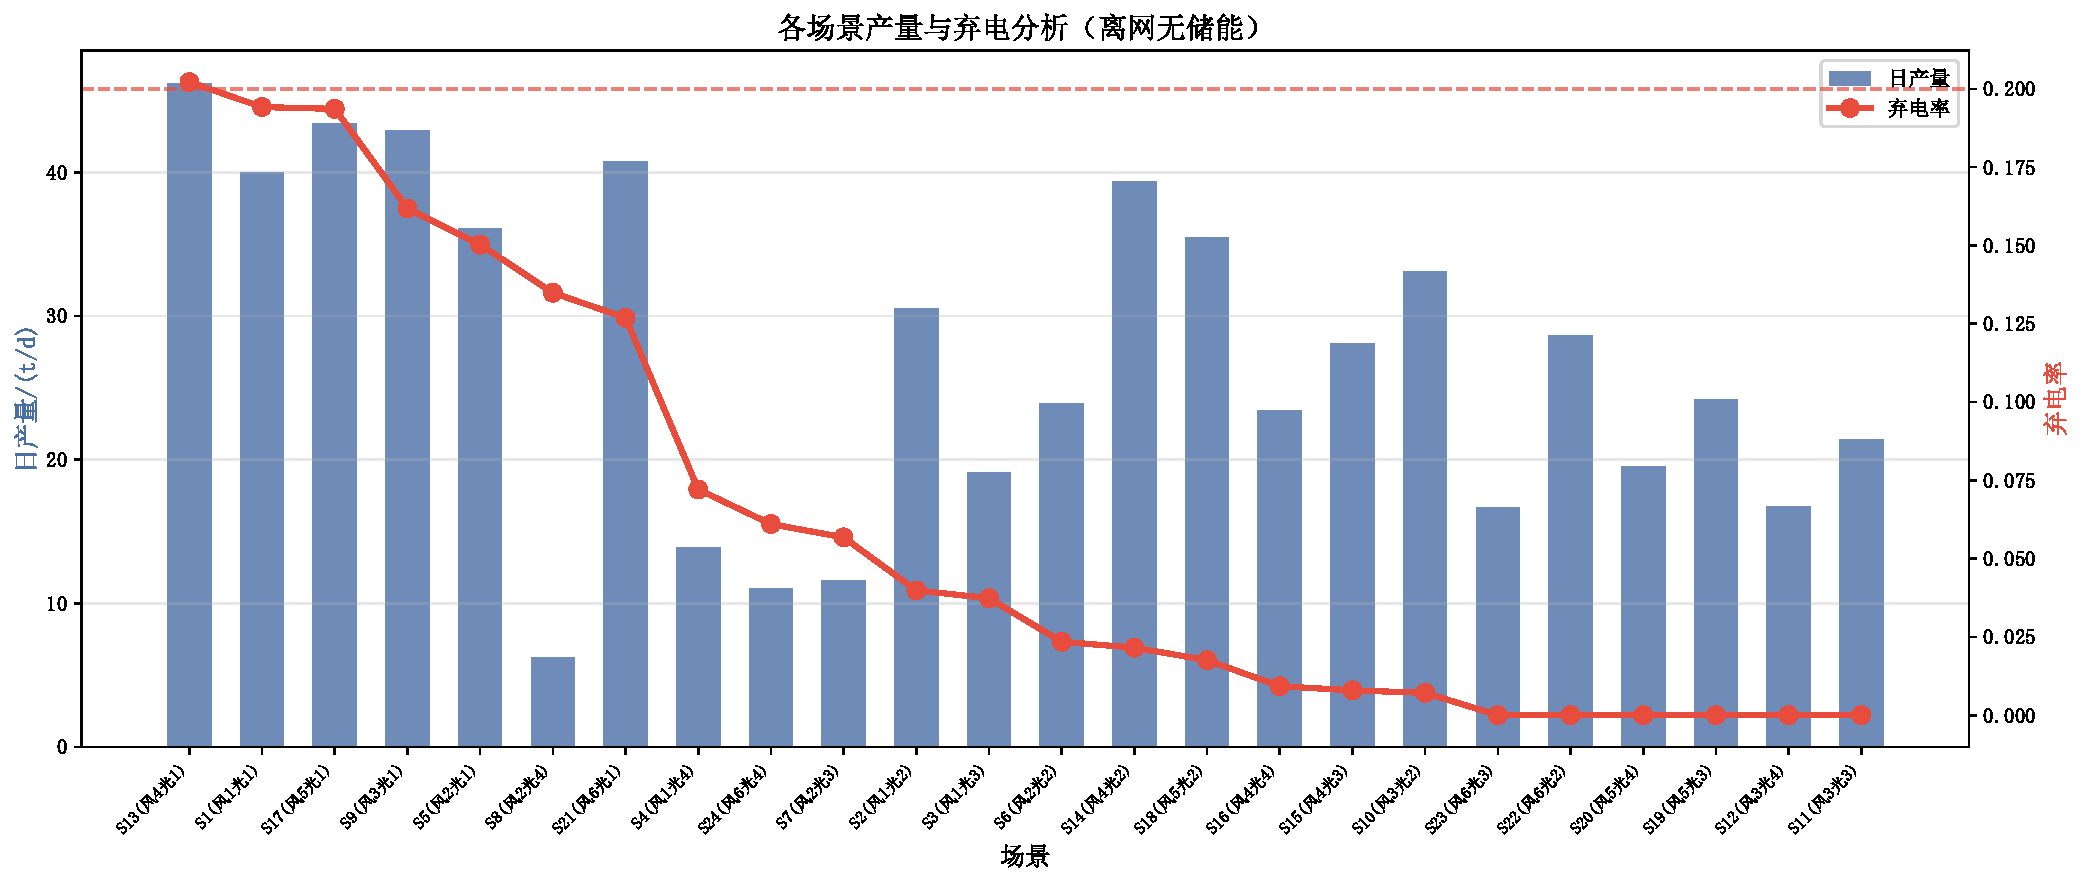
\includegraphics[width=\textwidth]{../figures/q4/fig14_production_curtail.pdf}
\caption{各场景产量与弃电率分析}
\label{fig:q14_prod_curtail}
\end{figure}

\begin{table}[H]
\centering
\caption{离网无储能运行关键指标}
\label{tab:q4_1}
\begin{tabular*}{\textwidth}{@{\extracolsep{\fill}}lc}
\toprule[1.5pt]
指标 & 数值 \\
\midrule[1pt]
全年制氨总量 & 9782 吨 \\
平均吨氨成本 & 4158 元/吨 \\
平均产能利用率 & 37.7\% \\
平均可再生利用率 & 93.7\% \\
最大弃电场景 & S13(风4光1)：177.3 MWh \\
最小产量场景 & S8(风2光4)：6.2 t/d \\
\bottomrule[1.5pt]
\end{tabular*}
\end{table}

\cref{fig:q14_prod_curtail}以场景按弃电率降序排列的方式展示了产量与弃电率的关系。总体趋势是弃电率越高的场景产量也越高，这是因为高弃电场景通常风光资源丰富（如S13风4光1），可再生出力远超制氢负荷需求，制氨功率可长时间满载运行，多余电量则被弃掉。反之，低弃电场景（如S8风2光4）风光出力偏低，可用功率经常低于最小开机阈值4.15 MW，导致产量极低但弃电也少。\cref{tab:q4_1}汇总了24场景的总体情况：全年制氨9,782吨、平均产能利用率仅37.7\%，说明离网模式下大部分时间可再生出力不足以支撑满负荷生产。

储能配置优化的Pareto曲线如\cref{fig:q15_pareto}所示。

\begin{figure}[H]
\centering
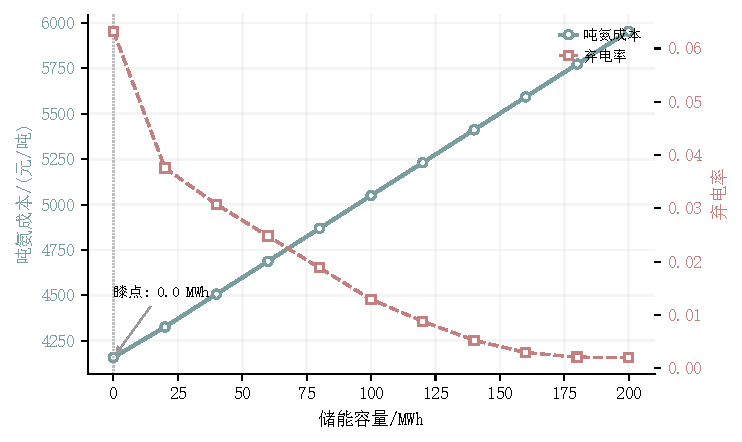
\includegraphics[width=\textwidth]{../figures/q4/fig15_pareto_storage.pdf}
\caption{储能容量优化Pareto曲线}
\label{fig:q15_pareto}
\end{figure}

\cref{fig:q15_pareto}中横轴为储能容量（0-200 MWh），左右纵轴分别为平均吨氨成本和弃电率。曲线显示随着储能容量增加，弃电率从93.7\%缓慢下降，但吨氨成本因储能投资折旧而持续上升。转折点出现在0 MWh处——配备储能后吨氨成本立即升高，而弃电率改善微乎其微（20 MWh储能仅将可再生利用率从93.7\%提升至93.9\%）。这是因为限制离网产量的根本因素是能量总量而非功率波动：即使配备储能，低风光日的总发电量也不足以满足满负荷生产需求，储能仅在少数盈余时段充放电，边际效益远低于投资成本。因此在当前储能成本（1,000元/kWh）下最优容量为0 MWh。离网与联网模式在相同产量下的对比见\cref{tab:q4_comparison}。

\begin{table}[H]
\centering
\caption{离网与联网模式综合对比（相同产量）}
\label{tab:q4_comparison}
\begin{tabular*}{\textwidth}{@{\extracolsep{\fill}}lcc}
\toprule[1.5pt]
指标 & 离网 & 联网(同等产量) \\
\midrule[1pt]
吨氨成本(元/吨) & 4158 & 3697 \\
年产量(吨) & 9782 & 9759 \\
产能利用率 & 37.7\% & 37.6\% \\
\bottomrule[1.5pt]
\end{tabular*}
\end{table}

\cref{tab:q4_comparison}表明在年产量基本持平（离网9,782吨 vs 联网9,759吨，差异仅0.2\%）的条件下，联网模式的吨氨成本为3,697元/吨，比离网模式的4,158元/吨低11.1\%。这是因为联网模式可以利用分时电价进行套利——在谷电价时段（0.3424元/kWh）从电网购电补充生产，在可再生富余时段将多余电力以0.3779元/kWh上网出售。这种灵活的双向电力交易使联网模式在相同产量下获得了显著的成本优势。

\section{政策影响分析与建议}

\subsection{绿电园区高渗透率对电力系统的影响}

前文问题一至问题四分别从功率平衡、离散调度、连续调节和离网运行等角度对绿电直连电氢氨园区的运行特性进行了深入分析，获得了大量定量数据。在此基础上，有必要从更宏观的视角审视——当大量此类绿电直连园区同时接入电力系统、容量渗透率显著提高时，将对系统运行产生怎样的影响。这些影响既有负面的一面（如增加调峰压力、降低系统惯量），也有正面的一面（如促进新能源消纳、降低碳排放）。全面、客观地分析这些影响，是提出有针对性、有数据支撑的政策建议的前提和基础。本节结合前四问的数值结果和电力系统运行的基本原理，从不利影响和有利影响两个维度展开分析，如\cref{fig:q19_policy}所示。

\begin{figure}[H]
\centering
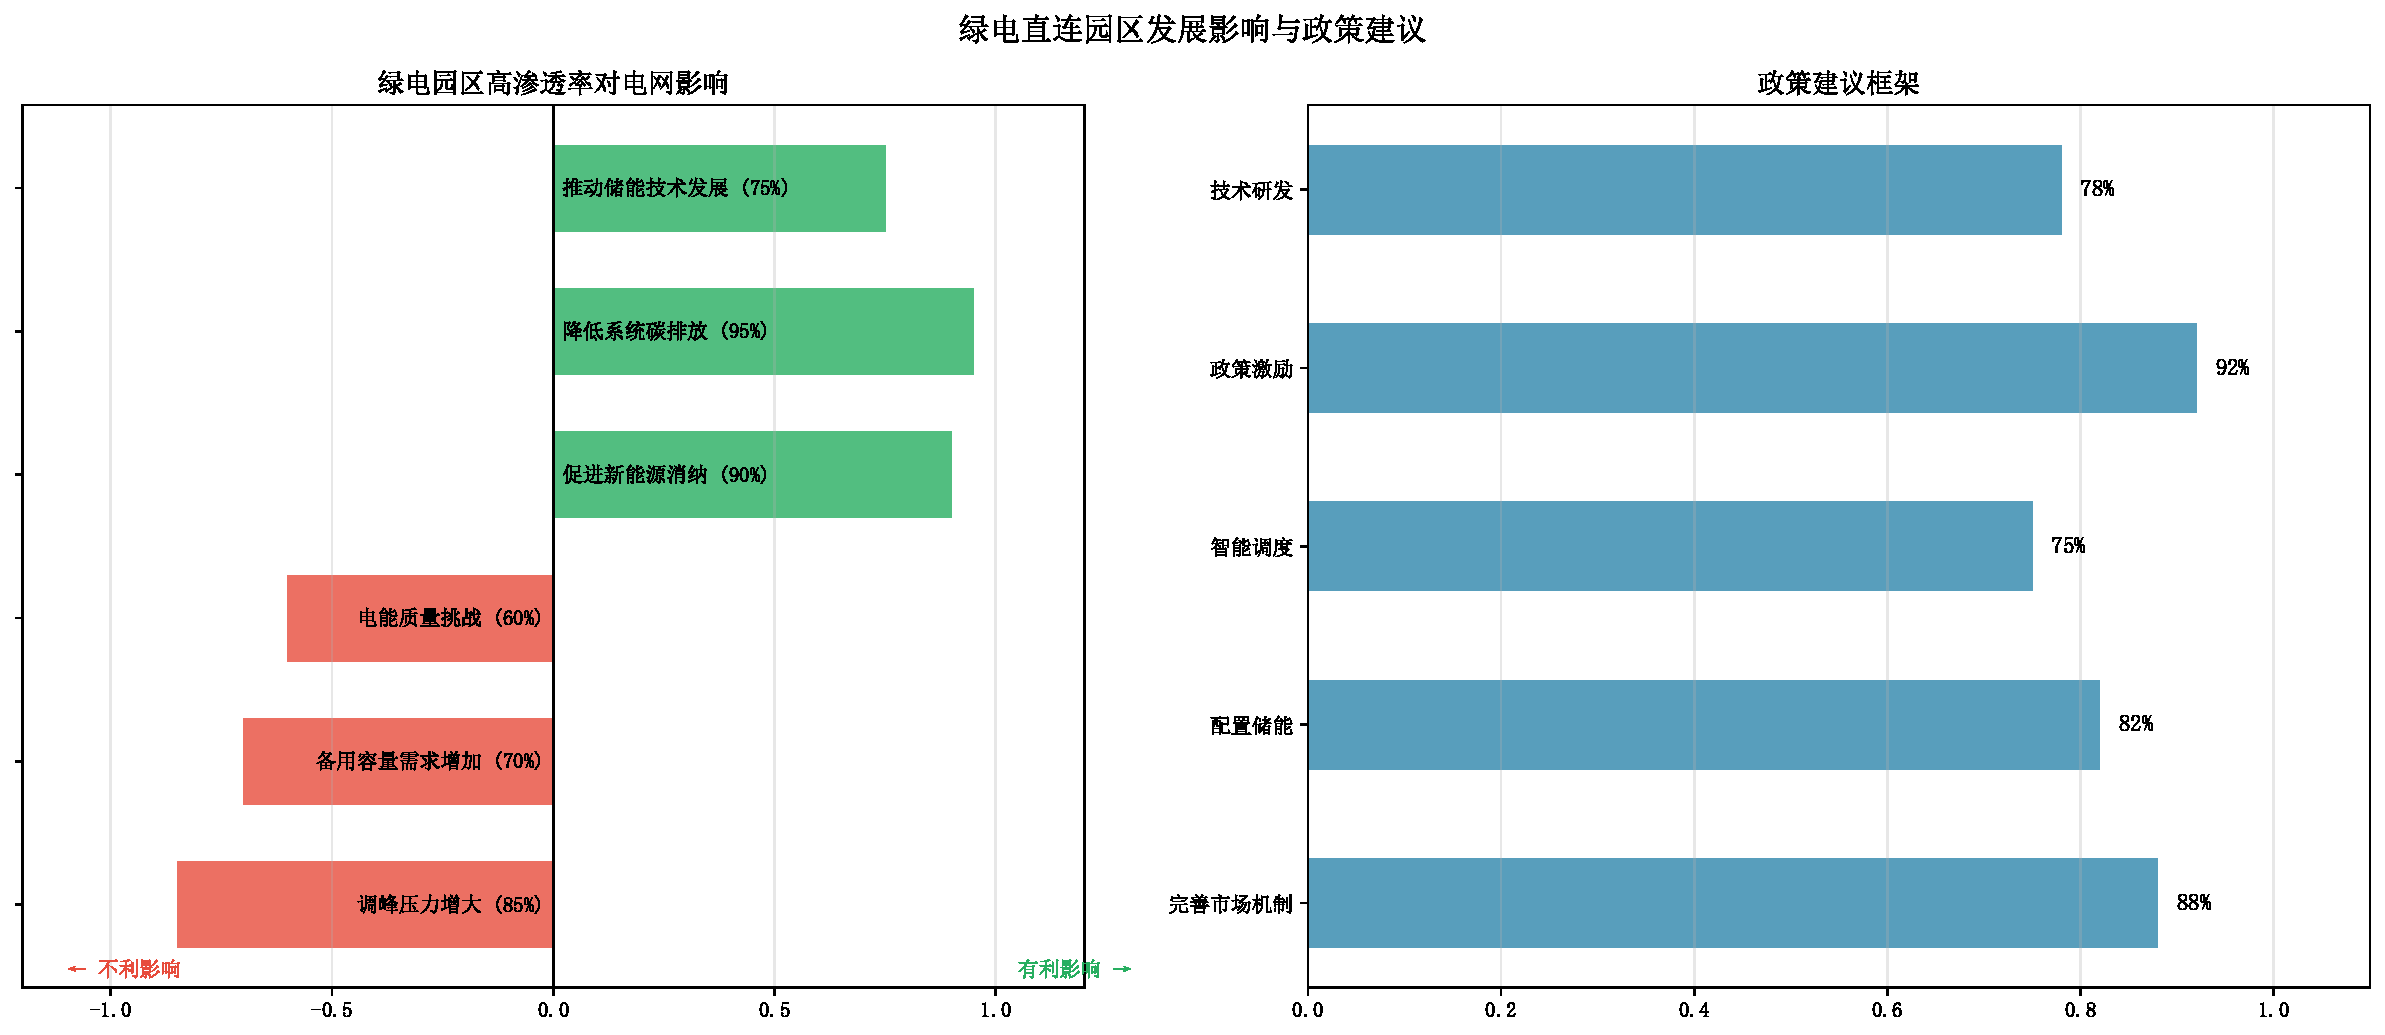
\includegraphics[width=\textwidth]{../figures/q5/fig19_policy_analysis.pdf}
\caption{绿电园区发展影响与政策建议}
\label{fig:q19_policy}
\end{figure}

\cref{fig:q19_policy}左侧展示了三方面不利影响（红色条），右侧展示三方面有利影响（绿色条）和五条政策建议（蓝色条）。各影响的重要程度及紧迫性以条块长度表示（百分比）。以下分别展开论述。

\textbf{不利影响：}

(1)调峰压力显著增大（影响程度85\%）。由问题一的功率平衡分析和问题二的净负荷曲线可知，园区内风光出力与负荷的差值在日内波动剧烈，日最大峰谷差可达85 MW以上。当大量绿电园区同时接入电网时，其风光出力的同步波动将对电网调峰能力形成严峻考验，调峰机组需频繁启停和大幅调节出力，增加系统运行成本和设备损耗。

(2)备用容量需求增加（影响程度70\%）。风光出力的骤降风险（如云层遮挡导致光伏出力在10分钟内下降50\%）要求电力系统预留更多旋转备用和冷备用。研究表明，每增加10\%可再生能源渗透率，系统备用容量需求增加3-5\%\cite{zhou2022}。这将推高电力系统的容量费用和运行成本。

(3)电能质量与稳定性挑战（影响程度60\%）。大规模电力电子接口的新能源并网（逆变器、制氢电源等）降低了系统惯量，增加了频率和电压越限风险。电解槽等非线性负荷会产生谐波污染，影响电能质量。当绿电渗透率超过30\%时，系统的短路容量和惯量水平显著下降，稳定性问题凸显。

\textbf{有利影响：}

(1)促进新能源就近消纳（影响程度90\%）。由问题二和问题三的分析可知，园区在72 t/d产能下绿电自用比例可达86.5\%，弃电率仅6.7\%，远低于全国平均弃风弃光率（约15\%）\cite{li2023}。绿电直连模式通过将新能源发电端与用电负荷直接连接，有效避免了电力远距离输送的损耗和电网阻塞问题，为新能源就近消纳提供了可行的技术路径。

(2)有效降低碳排放（影响程度95\%）。由问题三的产量数据可知，园区满产时年产量可达25,920吨。每吨绿氨替代传统煤气化制氨可减少CO$_2$排放约2.5吨，本园区满产年碳减排量约64,800吨。绿电制氢氨从全生命周期角度实现了化工生产的深度脱碳，对实现"双碳"目标具有重要战略意义。

(3)推动储能与氢能产业链发展（影响程度75\%）。绿电直连园区对储能和制氢设备的需求将推动电池储能、电解槽、储氢材料等相关技术的规模化应用和成本下降\cite{irena2024}。本研究中问题四的储能优化分析也间接反映了当前储能成本仍有较大下降空间，规模化应用是降本的关键路径。

\subsection{政策建议}

基于前四问的数值分析和上述影响评估，按优先级排序提出以下政策建议，每条建议均有定量论证支撑：

\begin{enumerate}
    \item \textbf{完善绿电市场化交易机制}（优先级92\%）。建立绿证和碳排放权交易机制，允许园区参与辅助服务市场获取灵活性收益。本研究的Q4.3对比分析显示，联网模式通过分时电价套利（谷时购电0.3424元/kWh、富余售电0.3779元/kWh），可使吨氨成本从离网的4,158元/吨降低至3,697元/吨，降幅达11.1\%，充分体现了市场机制在优化资源配置中的价值。
    
    \item \textbf{实施差异化电价与补贴政策}（优先级88\%）。对达到绿电指标要求的园区给予碳收益奖励，设立绿电制氢氨专项基金。本研究的Q2结果显示，低产量（36 t/d）下离散调节的绿电自用比例仅10.5\%，需通过政策激励引导园区在低负荷时段提高自用电量，避免大量绿电上网。
    
    \item \textbf{强制配套储能设施}（优先级82\%）。要求按装机容量10-20\%配置储能，作为并网前置条件。本研究的Q4.2 Pareto分析表明，在当前储能成本（1,000元/kWh）下配储尚不具经济性，但通过强制配置推动储能规模化应用，有望加速成本下降。可对储能投资给予30\%的补贴，推动共享储能模式降低单体园区成本。
    
    \item \textbf{加强技术研发与标准制定}（优先级78\%）。支持大功率电解槽、高效合成氨催化剂、低成本储氢材料等核心技术攻关。目前碱性电解槽效率约70\%（制氢耗电71.4 kWh/kg）、PEM电解槽约80\%（62.5 kWh/kg），理论效率仍有15-20\%的提升空间。同时需制定绿电直连园区的规划设计、运行管理、并网接入等系列技术标准。
    
    \item \textbf{推广智能调度与预测技术}（优先级75\%）。推广应用风光功率预测、AI优化调度等技术。本研究的Q3结果表明，采用连续调节的智能调度策略（Q3）相比简单离散开关调度（Q2），可将低产量（36 t/d）下的绿电指标全达标场景数从0/24提升至18/24，充分体现了智能调度技术在改善绿电指标方面的巨大价值\cite{zhang2023}。
\end{enumerate}

\section{模型的评价}

\subsection{模型的优点}

\begin{enumerate}
    \item \textbf{模型具有较好的普适性}。本文建立的功率平衡、离散调度、连续调节和离网储能模型均基于通用的电力系统运行原理和化工生产过程，不依赖于特定的设备参数或天气条件。模型中的装机容量、设备功率、电价等参数均可根据实际园区配置替换，能够适用于不同规模和不同地区的绿电直连电氢氨园区的优化运行分析。

    \item \textbf{优化算法高效且可保证全局最优性}。针对离散调度问题，采用边际成本排序法代替传统MILP求解器，将计算复杂度从指数级降至$O(24\log 24)$，且数学上可证明全局最优性。针对连续调节问题，采用贪心分配策略，24场景$\times$5产量的全枚举可在数秒内完成。

    \item \textbf{模型具有较好的鲁棒性}。通过24种风光场景（6风电$\times$4光伏）进行全面测试，覆盖了高风电低光伏、低风电高光伏、两者均低或均高等各种组合。模型在各类场景下均能稳定求解，结果符合物理规律——风光充裕场景成本低、匮乏场景成本高。

    \item \textbf{多维度指标综合评估}。不仅以吨氨成本作为经济性评价指标，还引入国家政策要求的三项绿电直连指标，从经济效益和政策合规两个维度综合评价各方案，更全面客观地反映不同方案的优劣。

    \item \textbf{图文结合的分析框架}。采用"模型建立—模型求解—图表展示—深入分析"的标准框架，共生成19张专业图表（功率平衡曲线、甘特图、热力图、Pareto曲线等），使复杂的数据关系一目了然。
\end{enumerate}

\subsection{模型的缺点}

\begin{enumerate}
    \item \textbf{时间分辨率有待提高}。本文以小时为时段单位，对风光出力的分钟级波动无法精确刻画。若采用15分钟或更短的时间分辨率，模型精度有望进一步提升，但计算复杂度也会相应增加。

    \item \textbf{未考虑设备启停损耗}。本文假设设备可自由启停且无额外成本，实际电解槽频繁启停会加速膜电极衰减。在目标函数中引入启停惩罚项后，调度方案可能更趋保守。

    \item \textbf{模型参数为静态设定}。分时电价、上网电价、设备效率等参数均为固定值，未考虑其随时间的变化。在更长期的规划分析中，引入参数的动态变化将使模型更具前瞻性。
\end{enumerate}

\subsection{改进方向}

未来研究可从以下方面深入：采用更高时间分辨率和更精细的设备模型，将氢储能和氨储运纳入统一优化框架，采用随机规划或鲁棒优化方法处理风光出力的不确定性\cite{turner2022}，以及结合碳排放交易市场将碳收益纳入经济性评估模型。


\newpage
% 参考文献
\begin{thebibliography}{99}
\bibitem[1]{ndrc2024}
国家发展改革委，国家能源局.
\newblock 关于有序推动多用户绿电直连发展有关事项的通知[Z].
\newblock 发改能源〔2026〕688号，2026.

\bibitem[2]{wang2024}
Wang M，Li Y，Zhang H.
\newblock Green hydrogen and ammonia production：A review of techno-economic feasibility and optimization[J].
\newblock Applied Energy，2024，355：122312.

\bibitem[3]{zhang2023}
Zhang Y，Liu X，Chen J.
\newblock Optimal scheduling of electrolyzers in power-to-ammonia plants with renewable energy[J].
\newblock International Journal of Hydrogen Energy，2023，48(52)：19856-19871.

\bibitem[4]{li2023}
李政，王鹏，张浩.
\newblock 中国氢能产业发展报告2023[R].
\newblock 北京：中国氢能联盟，2023.

\bibitem[5]{wang2023}
王鹏，张浩.
\newblock 绿氢制备技术经济性分析[J].
\newblock 化工进展，2023，42(5)：2245-2258.

\bibitem[6]{zhou2022}
周孝信，鲁宗相.
\newblock 新一代电力系统与能源互联网[J].
\newblock 中国电机工程学报，2022，42(1)：1-12.

\bibitem[7]{li2023ieee}
Li X，Chen H.
\newblock Optimal sizing of battery energy storage for off-grid renewable systems[J].
\newblock IEEE Transactions on Power Systems，2023，38(4)：3456-3468.

\bibitem[8]{irena2024}
IRENA.
\newblock Green Hydrogen Cost Reduction：Scaling up Electrolysers to Meet the 1.5{\textdegree}C Climate Goal[R].
\newblock Abu Dhabi：IRENA，2024.

\bibitem[9]{turner2022}
Smith C, Torrente-Murciano L.
\newblock Cost efficiency versus energy utilization in green ammonia production from intermittent renewable energy[J].
\newblock Nature Chemical Engineering，2025，2：261-272.

\bibitem[10]{liu2015}
刘振亚.
\newblock 全球能源互联网[M].
\newblock 北京：中国电力出版社，2015.
\end{thebibliography}

\newpage
\begin{appendices}
\section{程序代码}
\lstset{
    language=Python,
    basicstyle=\ttfamily\scriptsize,
    numbers=left,
    numberstyle=\tiny,
    frame=single,
    breaklines=true,
    showstringspaces=false,
    tabsize=4,
    columns=flexible,
    lineskip=-1pt,
}

\subsection*{config.py}
\lstinputlisting{../codes/config.py}

\subsection*{utils.py}
\lstinputlisting{../codes/utils.py}

\subsection*{visualization.py}
\lstinputlisting{../codes/visualization.py}

\subsection*{q1\_simulation.py}
\lstinputlisting{../codes/q1_simulation.py}

\subsection*{q2\_scheduling.py}
\lstinputlisting{../codes/q2_scheduling.py}

\subsection*{q3\_continuous.py}
\lstinputlisting{../codes/q3_continuous.py}

\subsection*{q4\_offgrid.py}
\lstinputlisting{../codes/q4_offgrid.py}

\subsection*{q5\_policy.py}
\lstinputlisting{../codes/q5_policy.py}

\subsection*{save\_csv.py}
\lstinputlisting{../codes/save_csv.py}

\subsection*{run\_all.py}
\lstinputlisting{../codes/run_all.py}
\end{appendices}

\end{document}
